\documentclass[10pt,twoside]{article}                           % Twoside para poder poner números en lados alternados

\usepackage[spanish]{babel}                                     % Configuración de lenguaje
\usepackage[a4paper,top=2cm,bottom=2cm,left=3cm,right=3cm,marginparwidth=1.75cm]{geometry}          % Configurar tamaño de pagina y márgenes
\usepackage{fancyhdr}
\usepackage[autostyle=true]{csquotes}
\usepackage[backend=biber,sorting=none]{biblatex}               % Paquete para bibliografía 
\addbibresource{Bibliografia.bib}                               % Llamo al archivo que contiene las referencias
\usepackage{amsmath}
\usepackage{amsfonts}
\usepackage{caption}                                            % Para que "Figura x.y" este en bold
\usepackage{graphicx}
\usepackage[hidelinks]{hyperref}                                % Para links entre partes del documento (hidelinks no le cambia el color a los links)
\usepackage{float}                                              % Permite forzar una posición para una figura
\usepackage[justification=centering,labelsep=space]{caption}    % Para poder centrar captions de figuras
\usepackage{gensymb}                                            % Símbolo de grados (\degree)
\usepackage{subfigure}                                          % Para poder usar subfiguras (logos de UNLP y FI juntos)
\usepackage{listings}                                           % Para poder incluir código
\usepackage{xcolor}                                             % Para poder definir colores  
\usepackage{enumitem}                                           % Para poder poner letras como items de listas
\usepackage{afterpage}                                          % Para poder insertar pagina en blanco
\usepackage{titlesec}                                           % Para cambiar tamaño de headers de secciones, subsecciones, etc.
\usepackage{titletoc}                                           % Para modificar el aspecto del índice (Table of Contents - ToC)
\usepackage[pagecolor=none]{pagecolor}                          % Para permitir usar colores de fondo en páginas
\usepackage{siunitx}                                            % Para notación científica (y unidades SI)
\usepackage{mathspec}                                           % Para tipografías custom, incluyendo ecuaciones (Incluye fontspec)

%-------------------------------------------------------------------------------------------------------%

% Definir todas las tipografías de mathspec

\setmainfont{Montserrat}                                        % Letra principal
\newfontfamily\Thin{Montserrat Thin}                            % Defino todos los pesos, también se pueden definir tipografías adicionales de la misma manera
\newfontfamily\ExtraLight{Montserrat ExtraLight}
\newfontfamily\Light{Montserrat Light}
\newfontfamily\Medium{Montserrat Medium}
\newfontfamily\SemiBold{Montserrat SemiBold}
\newfontfamily\Bold{Montserrat Bold}
\setmathrm[BoldFont = {Montserrat SemiBold Italic}]{Montserrat} 
\setmathfont(Digits,Latin){Montserrat}                          % Tipografía de matemática

% Comando para linea horizontal configurable que llene todo el espacio disponible 

\newcommand{\xfill}[2][1ex]{{%                                  % Si no hay texto antes del \xfill, hay que agregarle algun caracter como "\tiny\ " para que compile
  \dimen0=#2\advance\dimen0 by #1
  \leaders\hrule height \dimen0 depth -#1\hfill%
}}

% Comando para pagina en blanco sin numero de hoja

\newcommand{\ncblankpage}
{                          
    \null
    \thispagestyle{empty}
    \addtocounter{page}{-1}                         % No aumenta el contador de páginas
    \newpage
}



\newcommand{\blankpage}                             % Aumenta el contador de páginas
{                          
    \null
    \thispagestyle{empty}
    \newpage
}

% Definición de colores

\definecolor{AzulFI}{rgb}{0, 0.394, 0.645}                  % 0064A5
\definecolor{AzulFI_dark}{rgb}{0, 0.2353, 0.3882}           % 003C63
\definecolor{AzulFI_darker}{rgb}{0, 0.196, 0.3216}          % 003252
%\definecolor{codegreen}{rgb}{0,0.6,0}
%\definecolor{codegray}{rgb}{0.5,0.5,0.5}
%\definecolor{codepurple}{rgb}{0.58,0,0.82}
%\definecolor{backcolour}{rgb}{0.95,0.95,0.92}

% Estilo del header y footer

\pagestyle{fancy}

\renewcommand{\sectionmark}[1]{\markright{#1}}                          % Borra el numero de sección de \rightmark            
\renewcommand{\subsectionmark}[1]{}                                     % No marca las subsecciones

% Estilo nuevo
\fancyfoot[CO]{\SemiBold%
    \rule[-0.2em]{1pt}{1.1em}\hspace{0.5em}%
    \color{AzulFI_dark}Tomás Tavella\hspace{0.5em}\normalcolor\rule[-0.2em]{1pt}{1.1em}%
    \hspace{-0.05em}\xfill[0.6ex]{1pt}\hspace{-0.05em}%
    \rule[-0.2em]{1pt}{1.1em}\color{AzulFI_dark}\hspace{0.5em}\thepage\normalcolor\hspace{0.5em}\rule[-0.2em]{1pt}{1.1em}%
}

\fancyfoot[CE]{\SemiBold%
    \rule[-0.2em]{1pt}{1.1em}\hspace{0.5em}\color{AzulFI_dark}\thepage\hspace{0.5em}\normalcolor\rule[-0.2em]{1pt}{1.1em}%
    \hspace{-0.05em}\xfill[0.6ex]{1pt}\hspace{-0.05em}%
    \rule[-0.2em]{1pt}{1.1em}\color{AzulFI_dark}\hspace{0.5em}Tomás Tavella\normalcolor\hspace{0.5em}\rule[-0.2em]{1pt}{1.1em}%
}

\fancyhead[C]{\SemiBold%
    \rule[-0.2em]{1pt}{1.1em}\hspace{0.5em}\scshape\color{AzulFI_dark}Capítulo \thesection\normalcolor\hspace{0.5em}\rule[-0.2em]{1pt}{1.1em}%
    \hspace{-0.05em}\xfill[0.6ex]{1pt}\hspace{-0.05em}%
    \rule[-0.2em]{1pt}{1.1em}\color{AzulFI_dark}\hspace{0.5em}\rightmark\normalcolor\hspace{0.5em}\rule[-0.2em]{1pt}{1.1em}%
    }

\fancyhead[R,L]{}

\renewcommand{\headrulewidth}{0pt}
\setlength{\headheight}{12.60013pt}

\fancypagestyle{plain}{
    \fancyhead[L,C,R]{}
    %\fancyfoot[C]{}                                                    % Sólo va con el estilo viejo
    \renewcommand{\headrulewidth}{0pt}                                  % Para que no haya linea horizontal de encabezado en las páginas de índice y título de sección
}

% Parametros para setear como se muestra el codigo

\lstdefinestyle{mystyle}{                       
    backgroundcolor=\color{backcolour},
    commentstyle=\color{codegreen},
    keywordstyle=\color{magenta},
    numberstyle=\tiny\color{codegray},
    stringstyle=\color{codepurple},
    basicstyle=\ttfamily\scriptsize,
    breakatwhitespace=false,         
    breaklines=true,                 
    captionpos=b,                    
    keepspaces=true,                 
    numbers=left,                    
    numbersep=5pt,                  
    showspaces=false,                
    showstringspaces=false,
    showtabs=false,                  
    tabsize=4
}

\lstset{style=mystyle}

% Macro para divisores horizontales

\newcommand{\divider}                           
{
\begin{center}
    \hrulefill
\end{center}
\vspace{0.25cm}
\normalsize
}

% Macro para comillas

\newcommand{\quotes}[1]{``#1''}                 % Comando para double quotes

% Números de figura y ecuación por seccion (1.1 , 2.1, etc.)

\numberwithin{figure}{section}                  % Numeros de figura por seccion
\numberwithin{equation}{section}                % Numeros de ecuacion por seccion

% Definir formato de titulos de secciones y subsecciones

\titleformat{\section}[display]                                     % display permite el numero en linea separada del nombre
{\raggedright\color{AzulFI_dark}\scshape\Bold\Huge\centering}       % Formato del título de seccion
{\normalcolor\tiny\ \Huge\xfill[8pt]{1pt}\rule[-0.2em]{1pt}{1.1em}\hspace{0.5em}\color{AzulFI_dark}\thesection\normalcolor\hspace{0.5em}\rule[-0.2em]{1pt}{1.1em}\xfill[8pt]{1pt}\tiny\ }{0.5em}{}       % Formato del número de seccion

\titleformat{\subsection}[hang]{\raggedright\color{AzulFI_dark}\scshape\LARGE\Bold}{\thesubsection\quad}{0.5em}{}                      % Se agrega raggedright a todos para que no separe palabras en dos cuando tiene que hacer un line break

\titleformat{\subsubsection}[hang]{\raggedright\color{AzulFI_dark}\scshape\Large\SemiBold}{\thesubsubsection\quad}{0.5em}{}
\titleformat{\paragraph}[hang]{\raggedright\color{AzulFI_dark}\large\SemiBold}{}{0.5em}{}
\titleformat*{\subparagraph}{\raggedright\SemiBold}

% Formato de captions de figuras

\DeclareCaptionFormat{custom}
{%
    \SemiBold\scshape\color{AzulFI_dark} #1#2 \normalfont\normalcolor \textit{#3}                     % #1 es el número, #2 el separador y #3 el texto
}
\captionsetup{format=custom}

% Formato de Table of Contents (ToC)

\contentsmargin{1em}
\dottedcontents{section}[1.5em]{\large\vspace{0.4cm}\Bold\scshape\color{AzulFI_dark}}{1.5em}{0pc}      % Secciones en Bold en TableofContents
\dottedcontents{subsection}[4em]{\vspace{0.1cm}\Medium}{2.5em}{0.6pc}
\dottedcontents{subsubsection}[7.5em]{}{3.5em}{0.6pc}

%---------------------------------------------------------------------------------------------------------%
%------------------------------------------ Inicio de Documento ------------------------------------------%
%---------------------------------------------------------------------------------------------------------%

\begin{document}

    \nocite{*}                                                      % Se usa para que aparezcan todas la referencias del .bib sin tener que citarlas en el texto

    \newpagecolor{AzulFI}\afterpage{\restorepagecolor\blankpage}    % Página en blanco entre portada y agradecimientos

        \begin{titlepage}
        \begin{center}
            \vspace*{0.5cm}
            \Huge\scshape
            \color{white}
            \Bold{Diseño y Desarrollo de una Plataforma Experimental de Evaluación de Sistemas Híbridos Basados en Pilas de Combustible}    % Titulo
            \normalfont
            \\
            \vspace{0.5cm}
            \huge
            Proyecto Final                                       % Subtitulo
            \\
            %\divider
            \vspace{2cm}
            \Large\scshape
            \SemiBold{Autor:}
            \normalfont
            \\
            \large
            \vspace{0.2cm}
            Tomás Tavella
            \\
            N° 68371/4
            \\
            \vspace{1cm}
            \Large\scshape
            \SemiBold{Director:}
            \normalfont
            \\
            \vspace{0.2cm}
            \large
            Ing. Jorge Anderson Azzano
            \\
            \vspace{0.3cm}
            \Large\scshape
            \SemiBold{Co-Director:}
            \normalfont
            \\
            \vspace{0.2cm}
            \large
            Dr. Ing. Paul F. Puleston
            \\
            \vfill
            \begin{figure}[H]
                \centering
                \begin{subfigure}
                    \centering
                    
\includegraphics[width=0.25\textwidth]{Imagenes/UNLP.pdf}
                \end{subfigure}
                \begin{subfigure}
                    \centering
                    
\includegraphics[width=0.32\textwidth]{Imagenes/FI Invertido.png}
                \end{subfigure}
            \end{figure}
            \vspace{1cm}
            \SemiBold
            Facultad de Ingeniería
            \\
            Universidad Nacional de La Plata
            \vspace{1cm}
        \end{center}
    \end{titlepage}
    
    \addtocounter{page}{-1}
    \newpage 
    \thispagestyle{empty}                                           % Para que no se muestre el número de página al final (igual contribuye a la cuenta total)
    \afterpage{\ncblankpage}

    \huge
\scshape\color{AzulFI_dark}
\Bold{Agradecimientos}\\

\normalsize\normalfont\normalcolor
[Faltan los agradecimientos]

    \newpage
    \thispagestyle{empty}
    \afterpage{\blankpage}

    \huge
\scshape
\Bold{Resumen}\\

\normalfont\normalsize
Este trabajo consiste del estudio, diseño, implementación y validación de una plataforma experimental para la evaluación de sistemas híbridos de generación energía (SHGE) a partir de pilas o celdas de combustible de tipo PEMFC (\textit{Proton Exchange Membrane Fuel Cell}). Esta plataforma consiste en un sistema de conversión electrónico de tipo CC-CC conmutado y aislado, de topología puente completo; monitoreado mediante la medición de sus estados, y controlado por una excitación de tipo PWM (\textit{Pulse-Width Modulation}) provista por un DSC (\textit{Digital Signal Controller}) de alta performance. Este convertidor es requerido para poder adaptar la tensión variable que entrega una celda de combustible a una tensión de salida fija para conectar a un bus común de corriente continua.\\

En el desarrollo de este informe se detallan las tareas realizadas para cumplir este objetivo: el estudio y comprensión de las topologías de conversión CC-CC; la simulación de la topología elegida mediante herramientas de simulación circuitales; el diseño de circuitos auxiliares de excitación, sensado y protección; la implementación del sistema en una placa de circuito impreso mediante software EDA (\textit{Electronic Design Automation}); la programación de los algoritmos de control del sistema; y, finalmente la validación experimental de la plataforma.\\

\vspace{1cm}
\huge
\scshape
\Bold{Abstract}\\

\normalsize\normalfont
This work entails the study, design, implementation and validation of an experimental platform for the evaluation of hybrid energy generation systems based on Proton Exchange Membrane Fuel Cells (PEMFC). This platform incorporates a full-bridge isolated switched-mode DC-DC electronic converter, monitored via the measurement of its state variables, and controlled by a pulse-width modulated (PWM) signal, generated using a high-performance Digital Signal Controller (DSC). This converter provides the adaptation from the variable output voltage of the PEMFC to the fixed voltage of the common DC bus at the system output.\\

This report details the process through which the goals were achieved: study and understanding of the different DC-DC converter topologies, simulation of the selected converter topology using circuit simulation tools, design process of auxiliary circuits, including driver, sensing and protection circuits,  implementation of the system PCB (printed circuit board) through the use of electronic design automation (EDA) software, programming of system control algorithms, and experimental validation of the working platform.\\ 

    \newpage
    \afterpage{\blankpage} 
    \thispagestyle{plain}
    \tableofcontents
    \newpage

    \section{Introducción} \label{introduccion}
\AddToShipoutPictureBG*{
\includegraphics[width=\paperwidth,height=\paperheight]{Imagenes/Fondo Capitulo 1.pdf}}
\thispagestyle{plain}

\divider

Previo a comenzar con el diseño de la placa de circuito impreso, debemos introducir la plataforma que se tiene que plasmar en esta PCB, explicando brevemente su funcionamiento y los bloques principales y auxiliares que la componen. Se puede apreciar un diagrama de esta plataforma, separada en sus distintos bloques funcionales en la figura \ref{fig:plataforma}.\\

\begin{figure}[h]
    \centering
    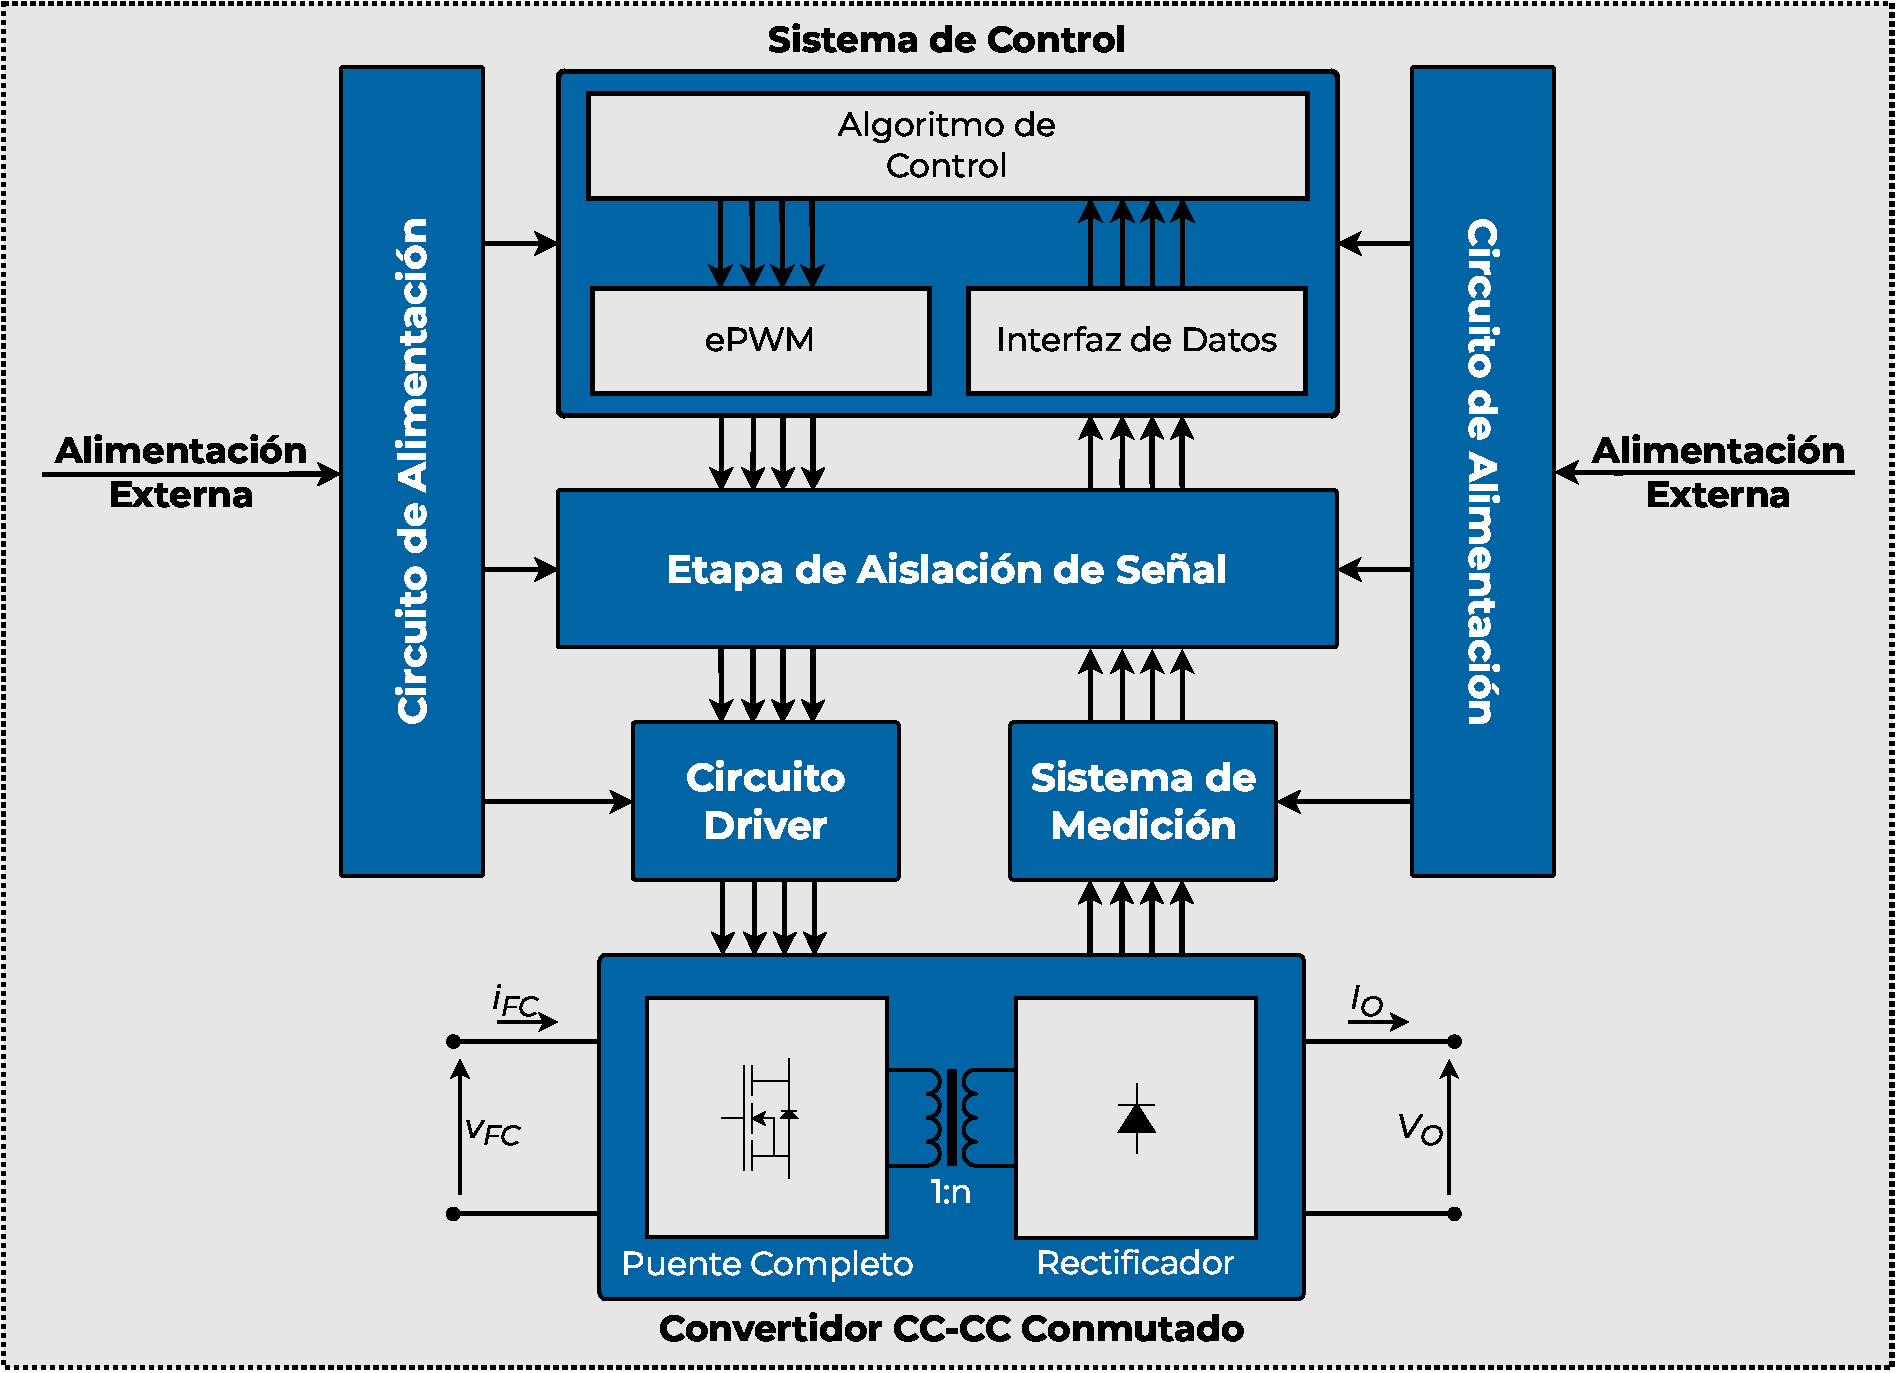
\includegraphics[scale=0.4]{Imagenes/Plataforma Detallada.pdf}
    \caption{Diagrama de la plataforma experimental de evaluación de celdas de combustible.}
    \label{fig:plataforma}
\end{figure}

Esta plataforma tiene como objetivo la adaptación de la interconexión de bloques en sistemas híbridos, sistemas complejos que combinan (o hibridan) múltiples módulos de generación y almacenamiento de energía, generalmente renovables, que luego se conectan a un bus de potencia de corriente continua (CC).\\

Particularmente, este sistema adapta el módulo de generación a partir de pilas de combustible para utilizar en un sistema híbrido, con una tensión de pila en la entrada $v_{FC}$ variable entre \SI[]{30}[]{\volt} y \SI[]{65}[]{\volt}, y una tensión de salida común fija de \SI[]{75}[]{\volt}. Para realizar esta la adaptación de estos niveles de tensión, se utilizó un convertidor CC-CC conmutado y aislado de tipo puente completo, que se regula mediante un sistema de control basado en un microcontrolador de tiempo real de la línea C2000 de Texas Instruments.\\

Previo a la realización de esta PPS, se trató el diseño circuital de la plataforma, construyendo los circuitos correspondientes a cada uno de los bloques que se muestran en la figura \ref{fig:plataforma}. Con estos circuitos diseñados, nos es posible pasar a su implementación en la placa de circuito impreso.\\
    
    \newpage

    \section{Análisis de la Plataforma} \label{analisis}
\AddToShipoutPictureBG*{
\includegraphics[width=\paperwidth,height=\paperheight]{Imagenes/Fondo Capitulo 2.pdf}}
\thispagestyle{plain}

\vspace{0.5cm}

\Large\scshape
\begin{center}
    {\Medium Planteo y estudio de la plataforma de evaluación\\ de celdas de combustible}
\end{center}
\normalfont
%\normalsize

\divider

En este capítulo, se realiza un detallado análisis de la Plataforma Experimental de Evaluación de Módulos de Celdas de Combustible de la figura \ref{diag_plataforma}, la cuál consiste en cuatro subsistemas o bloques distintos: 

\begin{itemize}
    \Medium \item Emulador de Celdas de Combustible
    \Medium \item Convertidor CC-CC Conmutado
    \Medium \item Sistema de Control
    \Medium \item Carga Electrónica Variable\\
\end{itemize}

\begin{figure}[h]
    \centering
    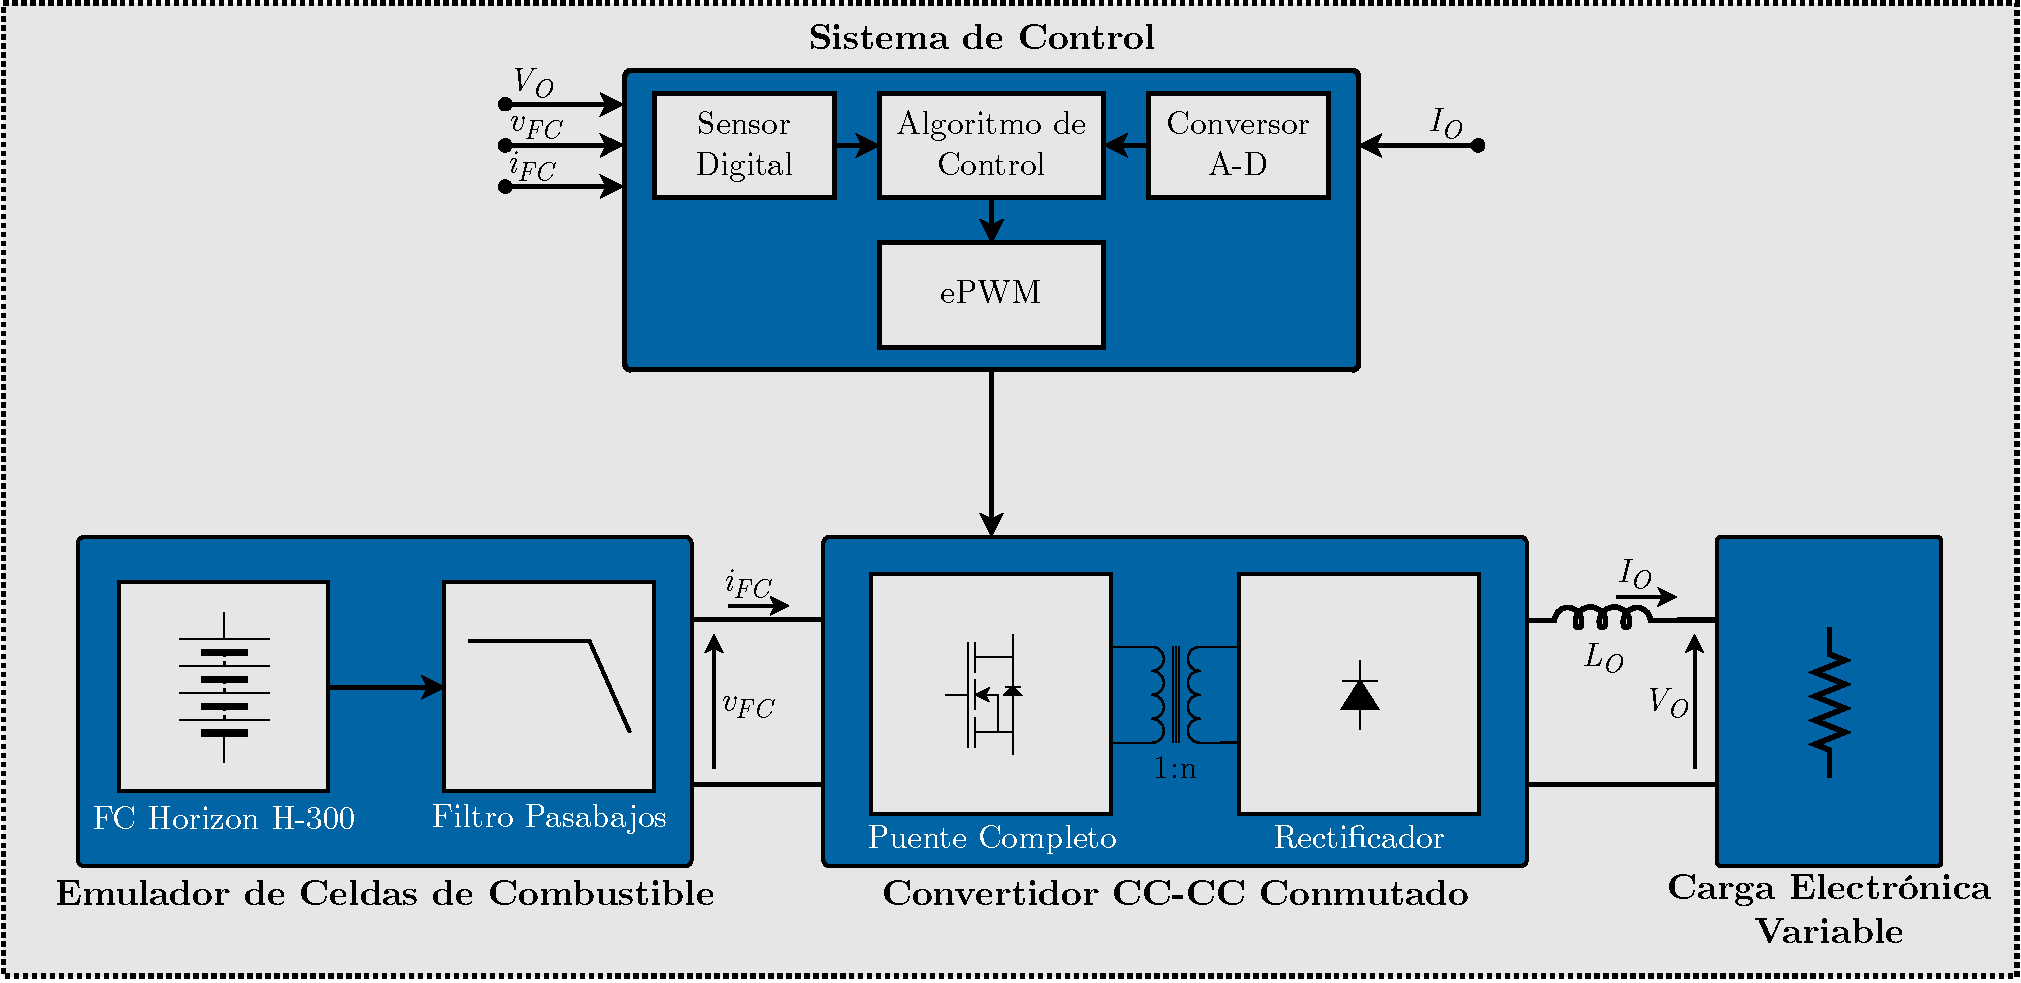
\includegraphics[scale=0.4]{Imagenes/Plataforma Experimental.pdf}
    \caption{Diagrama de la plataforma experimental de evaluación, con sus cuatro bloques principales.}
    \label{diag_plataforma}
\end{figure}

Esta plataforma, con sus distintos bloques, se encarga de evaluar la \textit{performance} de celdas de combustible conectadas a un sistema híbrido de generación. Con este fin, un emulador de celdas de combustible toma el puesto de celdas de combustible reales, y una carga electrónica variable se utiliza para simular cualquier tipo de condiciones de carga que se deseen en el bus de CC. Para poder conectar el emulador a la carga, se debe implementar un subsistema (Convertidor CC-CC Conmutado) que adapte los niveles de tensión de salida del emulador de celdas a la tensión fija de salida en la carga, adicionando un módulo de control que monitorea los estados del convertidor, y los controla mediante los disparos de las llaves del puente completo.\\

El principal objetivo de este proyecto es el diseño e implementación de la etapa de adaptación de tensión (es decir, el convertidor con su sistema de control), pero se hace un estudio detallado de todas los componentes de la plataforma, de manera de obtener un entendimiento más completo de todo el sistema. Por esta razón, a continuación se hace un análisis en profundidad de cada una de las partes individuales, comenzando por el emulador de celdas de combustible.\\

\subsection{Celdas de Combustible}

A pesar de que las celdas de combustible son una tecnología de hace más de un siglo y medio (desarrollada por primera vez por el físico galés Sir William Grove en 1842), hoy en día despiertan un particular interés en el campo de la generación renovable por su alta eficiencia, su dependencia en recursos obtenibles fácilmente de maneras ambientalmente amigables, y la generación de agua como único deshecho.\\

Por estas razones se eligió trabajar con esta tecnología, particularmente con el tipo de celda más común hoy en día, las Celdas de Combustible de Membrana de Intercambio Protónico o PEMFC (del inglés \textit{Proton Exchange Membrane Fuel Cell}), cuyo funcionamiento se profundiza más adelante.\\

\subsubsection{Principio de Funcionamiento}

Esencialmente, una celda de combustible es una celda galvánica o celda voltáica en la cual la energía libre de una reacción química redox (entre un combustible y un agente oxidante o \textit{comburente}) se convierte a energía eléctrica mediante una corriente y una diferencia de potencial.\textsuperscript{\cite{FC-FundAndAppl}} En nuestro caso particular, el combustible es el hidrógeno molecular ($H_2$), el agente oxidante es el oxígeno ($O_2$) abundante en la atmósfera, y los productos son la energía eléctrica y el agua ($H_2O$) según indica la siguiente ecuación química balanceada.

\begin{equation}\label{redox_celda}
    H_2\ +\ \frac{1}{2}O_2\ \longrightarrow\ H_2O
\end{equation}

La estructura interna de una celda de combustible, visible en la figura \ref{fuel_cell}, consta de un ánodo (electrodo negativo) al cual ingresan las moléculas de hidrógeno, un cátodo (electrodo positivo) en el que ingresa el oxígeno y se despide el agua, y un electrolito como como interfaz entre ánodo y cátodo. La carga es conectada entre el ánodo y el cátodo.\\

\begin{figure}[h]
    \centering
    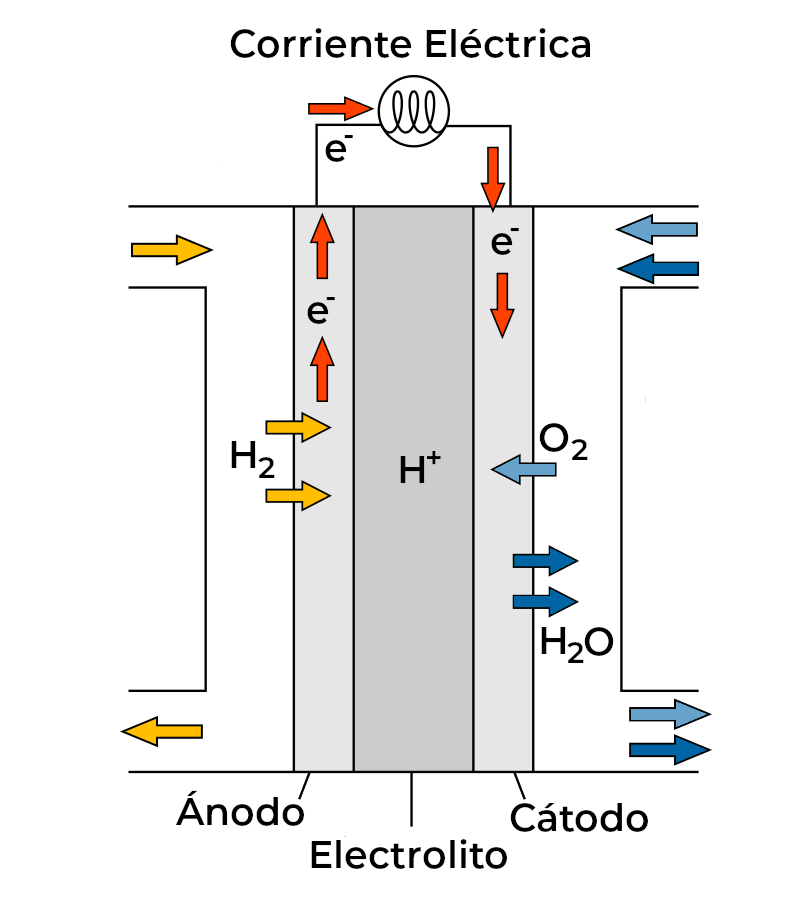
\includegraphics[scale=0.2]{Imagenes/Fuel Cell.png}
    \caption{Esquema ilustrativo de una celda de combustible, con todos sus componentes indicados.}
    \label{fuel_cell}
\end{figure}

La reacción redox de la ecuación \ref{redox_celda}, dentro de una celda de combustible como la del esquema, en realidad se separa en dos reacciones parciales distintas.

\begin{equation}\label{redox_anodo}
    H_2\ \longrightarrow\ 2H^{+}\ +\ 2e^-
\end{equation}

\begin{equation}\label{redox_catodo}
    2H^{+}\ +\ 2e^-\ +\ \frac{1}{2}O_2\longrightarrow\ H_2O
\end{equation}

De esta manera, alimentado simultáneamente el terminal negativo con combustible (hidrógeno) y el terminal positivo con oxidante (oxígeno) se producen las dos reacciones en las superficies de contacto del electrolito:

\begin{itemize}
    \item {\SemiBold En el ánodo ocurre la oxidación:} las moléculas de $H_2$ pierden sus electrones, bifurcándose los iones positivos de hidrógeno ($H^{+}$) por el electrolito y los electrones libres a través de la carga (ecuación \ref{redox_anodo}). Es una reacción exotérmica (libera calor) que resulta en el calentamiento de la celda.
    \item {\SemiBold En el cátodo ocurre la reducción:} los iones $H^{+}$ del electrolito, los electrones libres, y las moléculas de oxígeno reaccionan para formar como producto el agua (ecuación \ref{redox_catodo}).
\end{itemize}

Mediante este proceso electroquímico se generan dos corrientes distintas: una corriente interna de iones $H^{+}$ (cargas positivas) en el electrolito, desde el ánodo hacia el cátodo; y una corriente externa de electrones $e^-$ (cargas negativas) circulando por la carga, en el mismo sentido que la corriente de iones. Esta última corriente de electrones es la que nos resulta útil para poder alimentar algún tipo de carga.\\

\subsubsection{De Celda a Pila de Combustible}

Sin embargo, una celda de combustible individual como en la figura \ref{fuel_cell} no es capaz de entregar una diferencia de potencial lo suficientemente alta para la gran mayoría de las aplicaciones, con una tensión de celda común situada entre \SI{0.7}{\volt} y \SI{1.3}{\volt}, dependiendo de varios aspectos constructivos específicos de la celda.\\

Entonces, para obtener un dispositivo con una tensión de salida de niveles utilizables, esta tecnología generalmente se comercializa en forma de pilas o \textit{stacks} de celdas individuales conectadas en serie como se ve en la figura \ref{fuel_cell_stack}, generalmente de entre diez y cien celdas, cuya tensión es la suma de la tensión de cada celda que la compone.\\

Esto se logra, como dice su nombre, apilando todas las celdas de combustible para formar el \textit{stack}, utilizando placas de interconexión para conectar electrodos de polaridad opuesta de dos celdas aledañas (es decir, se conecta el ánodo de una celda con el cátodo de la siguiente); además de cumplir la función de aislar el combustible de una celda del agente oxidante de la celda contigua. Este es el tipo de conexionado de celdas más común, llamado \textit{Planar-Bipolar Stacking} o Apilado Planar-Bipolar.\textsuperscript{\cite{FCHandbook}}\\

\begin{figure}[h]
    \centering
    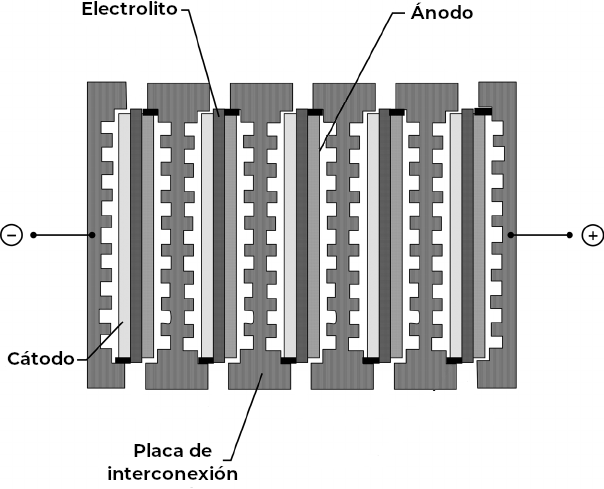
\includegraphics[scale=0.35]{Imagenes/Fuel Cell Stack.png}
    \caption{Diagrama interno de un stack de celdas conectadas por apilado planar-bipolar.}
    \label{fuel_cell_stack}
\end{figure}

\subsubsection{Aspectos Constructivos}

Habiendo repasado el principio básico de funcionamiento de las celdas de combustible, ahora se realizará una breve descripción de los aspectos constructivos de las mismas. La utilización de distintos materiales y composiciones de las partes que las componen derivan en distintos tipos de celdas, que, a pesar de funcionar bajo el mismo principio básico, poseen cada una sus ventajas y desventajas que las hacen más o menos apropiadas para distintas aplicaciones.\\

Como las reacciones químicas ocurren en superficies microscópicas dónde alguno de los electrodos está en contacto con el electrolito, generalmente los electrodos se fabrican de materiales porosos que aumentan la posible superficie de contacto entre ambas fases, acelerando las reacciones necesarias para producir energía. Sin embargo, en muchos casos, a temperaturas bajas los materiales de los electrodos no son capaces de producir la suficiente actividad electroquímica, por lo que suelen agregarse pequeñas cantidades de catalizador en las zonas de contacto para acelerar la reacción.\\

En tanto al electrolito, estos suelen estar hechos de materiales en estado líquido o sólido, dependiendo del tipo de celda, pero siempre deben tener una alta conductividad de iones positivos, de manera que los iones $H^{+}$ circulen solo por el elctrolito y no por el circuito externo. Adicionalmente, este material debe actuar de barrera física para evitar que se mezclen los flujos de combustible y comburente.\\

En tanto a la geometría de las celdas, se ha expermientado con una gran variedad de formas para los electrodos y electrolitos pero, hoy en día las pilas que se producen son mayormente planas, y en algunos casos tubulares.\\

\subsubsection{Tipos de Celdas}\label{tipos_celdas}

Hay muchas formas de clasificar las distintas tecnologías de celdas, pero en nuestro caso nos vamos a enfocar en la distinción más común, que es la clasificación según el material usado como electrolito. Hoy en día, hay seis tipos distintos de celdas segun electrolito, descritas a continuación, con una mayor profundización mayor en las del tipo PEMFC que se mencionaron anteriormente, ya que son este tipo de pilas las que nos interesa en nuestra aplicación particular.\\

\paragraph{Celda de Combustible Alcalina (AFC)}

Las AFC fueron las primeras celdas de combustible en ser desarrolladas, alrededor de 1960, e incluso hoy en día son las celdas de combustible con la mayor eficiencia eléctrica. Sin embargo, resultan poco viables, principalmente porque requieren gases muy puros para funcionar correctamente. Este requerimiento se da por el material electrolítico utilizado, el Hidróxido de Potasio (KOH) (en concentraciones de 85 \% para celdas de alta temperatura (\SI{250}{\celsius}), y entre 35 \% y 50 \% para celdas de baja temperatura (<\SI{120}{\celsius})), que reacciona facilmente con el dióxido de carbono que abunda en el aire, transformándose en $K_2CO_3$, destruyendo el electrolito y la celda en el proceso.\textsuperscript{\cite{FC-FundAndAppl}\cite{FCHandbook}}\\

\paragraph{Celda de Combustible de Membrana de Intercambio Protónico (PEMFC)}

Las PEMFC, también llamadas Celdas de Combustible de Electrolito Polimérico Sólido (SPEFC) son las celdas de combustible más utilizadas al día de hoy, habiendo conseguido usos en vehículos de combustible alternativo, lo que resultó en una gran inversión para su desarrollo. Estas celdas operan en rangos bajos de temperatura (entre \SI{65}{\celsius} y \SI{105}{\celsius}) y tienen un electrolito de estado sólido.\\
    
Este electrolito es una membrana de intercambio protónico: un membrana semipermeable que permite la conducción de protones y al mismo tiempo funcionando de aislación eléctrica entre los electrodos, y como barrera física para separar el combustible del comburente. Esta membrana solía fabricarse de sulfonato de poliéstireno, pero hoy en día se usan materiales basados en Politetrafluoretileno (PTFE) como el Nafion de DuPont o el Dow de Dow Chemical, que son más estables y poseen mayor conductividad de protones.\\

Su baja temperatura de operación, uso de materiales no exóticos, capacidad de altas densidades de corriente, resistencia a la corrosión dada por el electrolito sólido y bajo tiempo de arranque han hecho a las PEMFC la opción más popular al elegir un tipo de celda de combustible para utilizar. Sin embargo tiene sus desventajas, como el angosto rango de temperatura en el que requiere operar.\textsuperscript{\cite{FC-FundAndAppl}\cite{FCHandbook}}\\

Como esta es la tecnología de celda que nos interesa, se va a dedicar una sección para continuar más detalladamente la descripción de este tipo de celdas.\\

\paragraph{Celda de Combustible de Metanol Directo (DMFC)}

Las DMFC son un tipo especial de celdas de baja temperatura basadas en tecnología de las PEMFC, operando a temperaturas ligeramente mayores a estas. A diferencia de otras tecnologías, estas celdas utilizan metanol como combustible directamente, ahorrándose el paso de reformarlo a hidrógeno. El metanol es un combustible atractivo, ya que se puede producir a partir de gas natural o biomasa renovable y tiene una elevada energía específica.\textsuperscript{\cite{FC-FundAndAppl}\cite{FCHandbook}}\\

\paragraph{Celda de Combustible de Carbonato Fundido (MCFC)}

Las MCFC, desarrolladas a mediados del siglo XX, son celdas de combustible de alta temperatura de operación, entre \SI{600}{\celsius} y \SI{700}{\celsius}. Su electrolito esta compuesto de carbonatos fundidos de litio y sodio ($Li_2CO_3$ y $Na_2CO_3$) estabilizados por una matriz de fibras de alúmina ($Al_2O_3$). Suelen tener ánodos de níquel y cátodos de óxido de níquel.\\

Estas celdas pueden operar con una amplia variedad de combustibles, y, por su alta temperatura, no son tan susceptibles a contaminación por $CO$ o $CO_2$. Además, a diferencia del resto de las tecnologías, no son necesarios materiales catalizadores en los electrodos, ya que la combinación del níquel y las altas temperaturas proveen suficiente actividad electroquímica. Sin embargo, estas temperaturas generan problemas con los distintos materiales, reduciendo la vida útil de las celdas. Además tienen un electrolito altamente corrosivo y en estado líquido.\textsuperscript{\cite{FC-FundAndAppl}\cite{FCHandbook}}\\

\paragraph{Celda de Combustible de Óxido Sólido (SOFC)}

Las SOFC son celdas que llevan en continuo desarrollo desde mediados del siglo XX, y como indica su nombre, poseen un electrolito compuesto por un óxido en estado sólido, generalmente dióxido de zirconio ($ZrO_2$) o dióxido de cerio ($CeO_2$). Operan en rangos de temperatura muy elevados, de entre \SI{600}{\celsius} y \SI{1000}{\celsius}.\\

Estas celdas tienen la ventaja de tener un electrolito sólido, frenando la corrosión y permitiendo la fabricación en distintas geometrías. Además, todos sus materiales son de costo moderado. Como clara desventaja se encuentra la alta temperatura de operación, que trae problemas similares a los de las MCFC.\textsuperscript{\cite{FC-FundAndAppl}\cite{FCHandbook}}\\

\paragraph{Celda de Combustible de Ácido Fosofórico (PAFC)}

Las PAFC utilizan ácido fosfórico ($H_3PO_4$) con concetración de 100 \% estabilizado por una matriz basada en carburo de silicio ($SiC$) como electrolito, y operan en un rango de temperaturas entre \SI{150}{\celsius} y \SI{220}{\celsius}. Estas celdas son relativamente modernas y se destacan por su alta potencia, pudiendo llegar hasta \SI{20}{\mega\watt}, suficiente para una planta de generación intermedia.\\

Estas celdas son poco sensibles a contaminación de $CO$ y $CO_2$, y su baja temperatura de operación permite el uso de materiales comunes para su construcción. Sin enmbargo, su uso de ácido como electrolito requiere materiales más resistentes para sus electrodos.\textsuperscript{\cite{FC-FundAndAppl}\cite{FCHandbook}}\\

\subsubsection{Modelo Eléctrico de las PEMFC}

Las celdas del tipo PEM, como se describió en la anterior sección, son celdas de combustible de baja temperatura, con un electrolito sólido compuesto por una membrana de intercambio protónico. Para este trabajo se eligió este tipo de celdas por su extensivo desarrollo, fácil disponibilidad, bajo precio comparado con otras tecnologías, además de las ventajas ya mencionadas en la sección \ref{tipos_celdas}.\\

Entonces, debemos obtener un modelo eléctrico que caracterice a un stack de celdas tipo PEM, pudiendo luego implementar este modelo (en forma de una ecuación y curva tensión-corriente) en una simulación por computadora para evaluar el comportamiento del sistema completo.\\

Para comenzar, se debe encontrar una forma de cuantificar la energía química de las reacciones redox que ocurren dentro de la celda, pero esto no es tan sencillo como parece. Con este fin se utiliza el concepto de la \textit{energía libre de Gibbs}, que se podría definir como \quotes{la energía disponible para realizar trabajo externo} (en nuestro caso, el \quotes{trabajo externo} es mover los electrones por el circuito externo). Se define la \textit{energía libre de Gibbs de formación} $G_f$ como la energía de Gibbs tomando la energía cero a las condiciones normales de presión y temperatura.\\

Evidentemente, la energía entregada por la reacción es entonces la diferencia entre la energía $G_f$ de los productos y la energía $G_f$ de los reactivos, que por cuestiones de conveniencia se refieren a la energía por mol de producto y reactivo, indicado por una raya sobre la letra minúscula ($\bar{g_f}$).

\begin{equation}\label{delta_gibbs}
    \Delta\bar{g_f} = \bar{g_f}_{productos} - \bar{g_f}_{reactivos}
\end{equation}

Entonces, teniendo en cuenta la reacción redox de la ecuación \ref{redox_celda}, donde el producto es un mol de $H_2O$ y los reactivos son un mol de $H_2$ y medio mol de $O_2$, para nuestro caso la ecuación anterior resulta

\begin{equation}\label{delta_gibbs_celda}
    \Delta\bar{g_f} = \bar{g_f}_{(H_2O)} - \bar{g_f}_{(H_2)} - \frac{1}{2}\bar{g_f}_{(O_2)}
\end{equation}

Ahora, teniendo en cuenta que el trabajo eléctrico realizado es el producto de la carga por la tensión ($W_E=Q\cdot E$), y considerando un proceso sin irreversibilidades y con combustible y comburente puro, se puede decir entonces que el trabajo eléctrico es aproximadamente igual a la energía química entregada por la reacción de la celda, es decir que $W_E = \Delta\bar{g_f}$.\\

Lo que hace falta, entonces, es obtener la cantidad de carga que circula a través del circuito externo por cada mol de agua que se produce. Como se puede ver en las dos reacciones parciales de las ecuaciones \ref{redox_anodo} y \ref{redox_catodo}, por cada mol de $H_2O$ que se obtiene, dos átomos de hidrógeno pierden su electrón, y en consecuencia, dos electrones circulan a través de la carga. Entonces, si $e$ es la carga de un electrón (\SI{1.602e-19}{\coulomb}) y $N$ es el número de Avogadro (\num{6.022e-23}) que indica la cantidad de partículas en un mol, la carga por cada mol es

\begin{equation}\label{carga_mol}
    Q=-2\cdot Ne=-2\cdot F=\SI{192970}{\coulomb}
\end{equation}

Donde $F$ es la constante de Faraday, que indica la carga de un mol de electrones.\\

Reemplazando la ecuación \ref{carga_mol} en la expresión del trabajo eléctrico (recordando que es equivalente a $\Delta\bar{g_f}$), se obtiene la siguiente expresión de energía obtenida por mol de producto.

\begin{equation}\label{trabajo_elec}
    W_E=\Delta\bar{g_f}=-2F\cdot E
\end{equation}

Entonces, si despejamos la tensión de circuito abierto $E$ (es decir corriente nula) de la ecuación anterior, podemos obtener una expresión para esta tensión en función de la energía de Gibbs de formación de la reacción, que para una temperatura de \SI{80}{\celsius} de una celda tipo PEM típica es de \SI{-228.2}{\kilo\joule\per\mole}.\textsuperscript{\cite{FCSysExplained}}

\begin{equation}\label{tension_vacio}
    \boxed{E=-\frac{\Delta\bar{g_f}}{2F}=\SI{1.183}{\volt}}
\end{equation}

Con esta ecuación, por lo tanto, se puede obtener la {\Medium tensión de circuito abierto de celda} \textit{teórica} de una celda de combustible cualquiera; pero se debe tener en cuenta que este valor es ideal, y no tiene en cuenta múltiples factores que reducen la eficiencia (y la tensión de circuito abierto) del dispositivo: no es posible utilizar el 100 \% del combustible disponible, algunas dinámicas de las reacciones utilizan parte de la energía química generada, entre otros. Además, en este desarrollo no se consideró la variación de la energía libre de Gibbs con la presión y concentracion de gases.\\

\paragraph{Modelo Tensión-Corriente}

Sin embargo, esto no es suficiente para un análisis eléctrico completo del dispositivo. Ahora se deben describir las distintas partes de una curva típica de tensión-corriente de una celda de combustible de baja presión y temperatura (como las PEMFC), y al mismo tiempo presentar las ecuaciones que la describen para poder obtener el modelo eléctrico completo que se busca. Se puede ver esta curva típica en la figura \ref{V-I_celda}.\\

\begin{figure}[h]
    \centering
    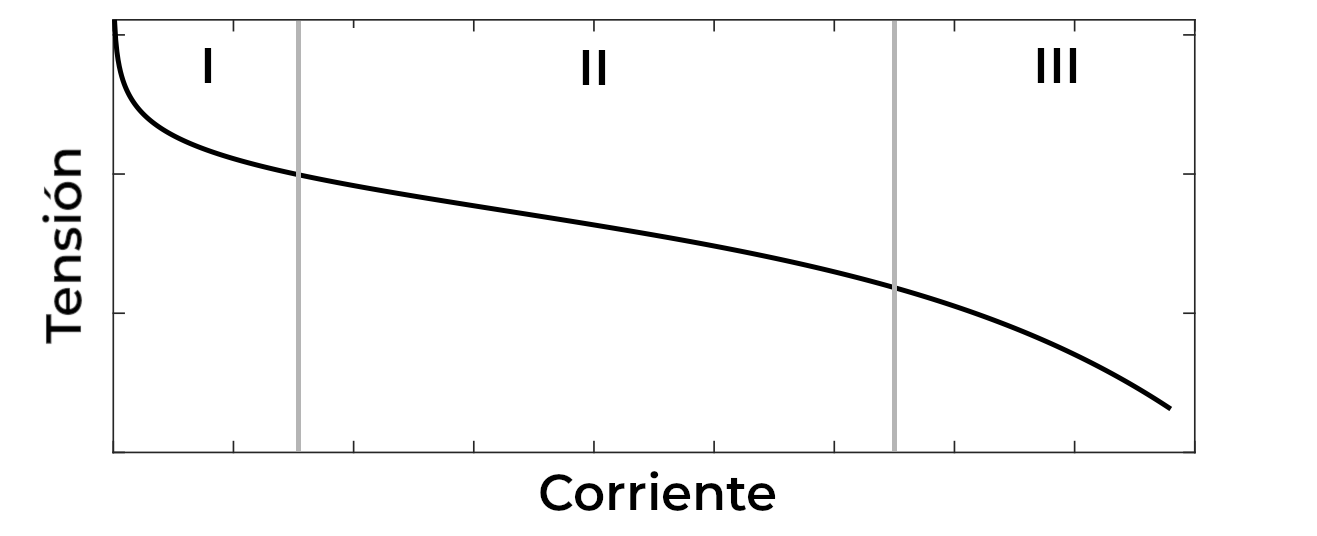
\includegraphics[scale=0.28]{Imagenes/Curva V-I Celda.png}
    \caption{Curva de tensión vs. corriente típica de una celda de combustible tipo PEM, con sus tres regiones marcadas.}
    \label{V-I_celda}
\end{figure}

En esta curva se pueden señalar tres regiones de pérdidas bien marcadas: la región de {\Medium pérdidas de activación (I)} cerca de corriente nula, seguida por la región de {\Medium pérdidas óhmicas (II)}, y finalmente, acercándose a la máxima corriente, la región de {\Medium pérdidas de concentración (III)}. Estas pérdidas se dan por algunas irreversibilidades de las reacciones que ocurren en la celda, que la alejan de su comportamiento ideal. A continuación se detallan estos componentes y se obtienen sus ecuaciones correspondientes.\\

\subparagraph{Región de Pérdidas de Activación (I)}

Como se puede ver, en la primera región hay una rápida caída de tensión de características no lineales. Esto ocurre por las llamadas \textit{pérdidas de activación}, que se generan por la lenta velocidad de reacción en las superficies de los electrodos para bajas densidades de corriente. Una porción de la tensión generada se pierde al generar la reacción electroquímica, que transfiere los electrones desde o hacia los electrodos.\\

La ecuación asociada este comportamiento, formulada empíricamente por el químico suiso Julius Tafel en 1905, es una ecuación que es describe la caída de tensión en un electrodo para una gran variedad de reacciones, incluida la rección redox de agua que nos interesa. La ecuación de Tafel relaciona la caída de tensión en un electrodo $\Delta V_{act}$ con la densidad de corriente $i$ que circula a través del mismo mediante una forma logarítmica.
    
\begin{equation}\label{perd_act}
    \Delta V_{act}=A\cdot \ln\left(\frac{i}{i_0}\right)
\end{equation}

La constante $i_0$ (llamada \textit{densidad de corriente de intercambio}) se puede considerar como la densidad de corriente para la cual la tensión de celda se comienza a alejar de la ideal de la ecuación \ref{tension_vacio}, y su valor aumenta mientras más rápida sea la reacción. En contraste, la constante $A$ que multiplica al logaritmo es mayor para una reacción electroquímica lenta.\\

En el caso particular del hidrógeno como combustible, las pérdidas se concentran casi únicamente en el ánodo (donde ocurre la oxidación), con la densidad $i_0$ del ánodo generalmente mas de \num{10000} veces mayor a la del cátodo, por lo que generalmente las pérdidas de activación de este último se pueden despreciar, teniendo en cuenta únicamente las del ánodo.\\

\subparagraph{Región de Pérdidas Óhmicas (II)}

Esta región es la que abarca el mayor rango de corrientes de celda, además de ser la más simple de modelar y entender. En este caso, las pérdidas se dan simplemente por la resistencia eléctrica al paso de corriente de ambos electrodos y la resistencia al paso de iones del electrolito, y por lo tanto, la caída de tension $\Delta V_{ohm}$ esta relacionada linealmente con la densidad de corriente $i$ mediante la Ley de Ohm.

\begin{equation}\label{perd_ohm}
    \Delta V_{ohm}=i\cdot r
\end{equation}

Donde $r$ debe ser la resistencia por unidad de área (\unit{\ohm\metre\squared}) si se trabaja con $i$ como densidad de corriente (\unit{\ampere\per\metre\squared}).\\

\subparagraph{Región de Pérdidas de Concentración (III)}
    
Esta última región de pérdidas viene dada, como dice su nombre, por la reducción de la concentración de combustible y comburente en el ánodo y cátodo respectivamente, condición que se ve exacerbada al trabajar con corrientes y cargas muy elevadas. Esta reducción en concentración se traduce a una reducción de la tensión de celda $\Delta V_{conc}$.\\

En general, el consenso es que no existe una única ecuación analítica que sea capaz de describir este comportamiento para cualquier caso. Entonces, hoy en día es muy común el uso de una ecuación de bases empíricas que, con la correcta elección de constantes, se ajusta muy bien al comportamiento real observado experimentalmente, y relaciona $\Delta V_{conc}$  exponencialmente con la densidad de corriente $i$.

\begin{equation}\label{perd_conc}
    \Delta V_{conc}=m\cdot e^{ni}
\end{equation}

Donde las constantes $m$ y $n$ suelen estar alrededor de \SI{3e-5}{\volt} y \SI{8e-3}{\cm\squared\per\milli\ampere} respectivamente.\\

Habiendo obtenido la ecuacion para la tensión irreversible (ecuación \ref{tension_vacio}) y las ecuaciones de cada una de las tres regiones (ecuaciones \ref{perd_act}, \ref{perd_ohm} y \ref{perd_conc}), se pueden combinar todas en una única expresión que modela la tensión de una celda para cualquier densidad de corriente:

\begin{equation}
    \begin{aligned}
        V_{celda} & = E - \Delta V_{act} - \Delta V_{ohm} - \Delta V_{conc}\\
                  & = E - A\cdot \ln\left(\frac{i}{i_0}\right) - i\cdot r - m\cdot e^{ni}
    \end{aligned}
\end{equation}

Sin embargo, todavía se pueden realizar algunas simplificaciones. Para la ecuación \ref{perd_act}, que expresa la caída de tension por activación, la densidad de corriente de intercambio $i_0$ es muy baja, mucho menor a la densidad de corriente $i$, por lo que esta ecuación se puede modificar de la siguiente manera:

\begin{equation*}
    \Delta V_{act} = A\cdot \ln(i) - A\cdot \ln(i_0)
\end{equation*}

Como el último término solo depende de $i_0$, que es un valor constante, se lo puede agrupar con la tensión irreversible $E$, para obtener una tensión de circuito abierto real y reversible $E_{oc}$.

\begin{equation}
    E_{oc} = E + A\cdot\ln(i_0)
\end{equation}

Vale aclarar que, al ser la densidad de corriente de intercambio una magnitud muy chica, al calcular su logaritmo natural se obtiene un número negativo, por lo que la tensión de circuito abierto reversible $E_{oc}$ resulta, como es esperable, menor la la tensión irreversible $E$. Entonces, la expresión final que describe la relación tensión vs. corriente de una celda de combustible se muestra en la siguiente ecuación.

\begin{equation}\label{v_celda}
    V_{celda}(i) = E_{oc} - A\cdot\ln(i) - i\cdot r - m\cdot e^{ni}
\end{equation}

Para obtener la tensión de una pila, solo es necesario multiplicar la tensión $V_{celda}$ por la cantidad de celdas $N$ del stack.

\begin{equation}\label{v_stack}
    \boxed{
    \highlight{V_{stack}(i) = NV_{celda}(i) = N\cdot (E_{oc} - A\cdot\ln(i) - i\cdot r - m\cdot e^{ni})}
    }
\end{equation}

\subsubsection{Emulador de Celdas de Combustible}

Esta plataforma se basa en la utilización de un modelo comercial particular de pila de combustible: el módulo H-300 de la serie H de pilas de combustible de Horizon Fuel Cell Technologies de la figura \ref{H300}. Esta es una pila de combustible de \SI[]{300}[]{\watt} enfriada por aire del tipo PEMFC, qur consiste en un stack de \num{60} celdas. Su desempeño nominal es de \SI[]{36}[]{\volt} de tensión a \SI[]{9}[]{\ampere} de corriente y tiene una tensión de circuito abierto de aproximadamente \SI[]{60}[]{\volt}.\textsuperscript{\cite{HSeriesBrochure}}\\

\begin{figure}[h]
    \centering
    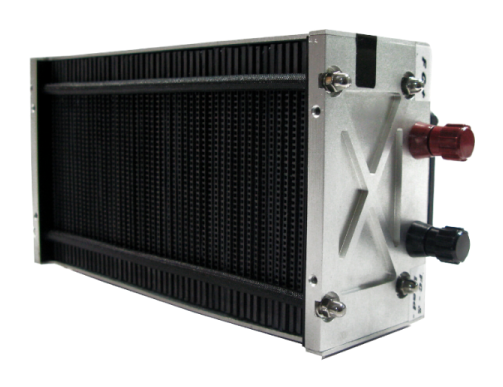
\includegraphics[scale=0.4]{Imagenes/Horizon H-300.png}
    \caption{Pila de combustible tipo PEMFC, modelo Horizon Fuell Cell Technologies H-300.}
    \label{H300}
\end{figure}

Sin embargo, dado que este módulo no está presente en el laboratorio, como reemplazo se utiliza un {\Medium módulo de emulación de pilas de combustible}. Este módulo permite la reproducción de una curva tensión-corriente de una pila en condiciones de trabajo controladas.\\

Este módulo consiste en un convertidor CC-CC conmutado de tipo reductor, (que se explicará mas adelante) que impone una tensión de salida en función de la corriente suministrada a través de un lazo de control. El modelo que utiliza para obtener la tensión de salida en función de la corriente es el que se se obtuvo en la ecuación \ref{v_stack} y en el gráfico de la figura \ref{V-I_celda}. El módulo se puede ajustar a distintos modelos de celdas mediante la variación de las constantes $N$, $E_{oc}$, $A$, $r$, $m$ y $n$. Los valores de la curva se almacenan en una tabla de \textit{look-up} implementada en un FPGA.\\

Adicionalmente a la característica tensión-corriente de la celda, este módulo permite simular el filtro pasabajos propio de la pila que se ve en el diagrama de la plataforma de la figura \ref{diag_plataforma}. Este filtro cumple la función de proteger a las celdas y evitar deterioro de las mismas mediante una reducción del rizado de corriente que puede generar la conmutación del convertidor.\textsuperscript{\cite{Argencon2018}}\\

\newpage

\subsection{Convertidor CC-CC Conmutado}

Un convertidor CC-CC es un dispositivo electrónico que tiene como objetivo convertir una tensión continua, generalmente no regulada (es decir que no es fija), $V_{in}$ a la entrada, a una tensión continua regulada $V_{out}$ de distinta magnitud a la salida, transfiriendo la mayor cantidad de energía posible de la entrada hacia la salida. Dependiendo del tipo de convertidor, esta tensión de salida puede ser menor, mayor o tanto menor como mayor a la tensión de entrada.\\

Estos convertidores son de interés para nuestra aplicación, ya que la tensión $V_{stack}$ que entrega la pila (ecuación \ref{v_stack}) es una tensión continua no regulada, que varía apreciablemente con la corriente demandada; mientras que a la salida se demanda una tensión fija y regulada $V_{bus}$ para conectar al bus de continua del sistema híbrido de la figura \ref{SHGE}.\\

Los convertidores CC-CC se suelen separar en dos principales categorías: los {\Medium reguladores lineales}, que consisten en un divisor resistivo con una resistencia variable implementada mediante un transistor (además de un diodo para regular la tensión de salida); y los {\Medium convertidores conmutados}, en los cuales uno o más transistores, actuando como llaves, son conmutados a alta frecuencia y junto con dispositivos que almacenan energía (como inductores y capacitores) producen una tensión continua a la salida.\\

Dado que para esta plataforma se utiliza un convertidor conmutado (principalmente por su gran ventaja en eficiencia energética), se enfocará el análisis únicamente en éstos; comenzando por una explicación de los conceptos básicos necesarios para comprender su funcionamiento.\\

\subsubsection{Conceptos Básicos}

Como se detalló más arriba, los convertidores CC-CC conmutados consisten, en su forma más básica, en una fuente de continua no regulada a la entrada; y un transistor (que puede ser BJT, MOSFET o IGBT) que, mediante una excitación en su tercer terminal, se conmuta entre los modos de alta impedancia e impedancia nula, actuando como llave abierta y llave cerrada respectivamente. La proporción del tiempo total de ciclo ($T_s$) en la que el transistor está conduciendo ($t_{on}$) se denomina {\Medium ciclo de trabajo} o {\Medium \textit{duty cycle}} y se suele simbolizar con la {\Medium letra \textit{D}}. Como se verá más adelante, este es un parámetro crucial para el funcionamiento de este tipo de convertidores, ya que controlándolo se puede variar el nivel de tensión y corriente de salida.\\

\begin{figure}[h]
    \centering
    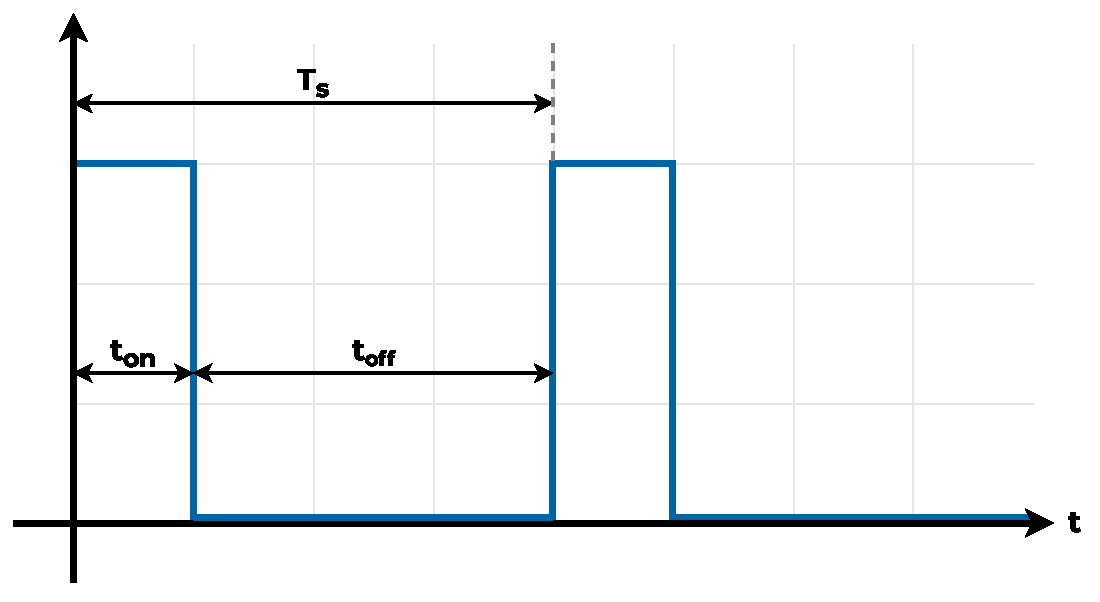
\includegraphics[scale=0.5]{Imagenes/Duty Cycle.pdf}
    \caption{Una forma de onda cuadrada con ciclo de trabajo $D$ del 25 \%.}
    \label{dutycycle}
\end{figure}

Los convertidores CC-CC conmutados se clasifican en dos grandes grupos, usando como criterio la existencia de aislación galvánica entre la entrada no regulada y la salida regulada:

\begin{itemize}
    \item {\SemiBold Convertidores No Aislados:} son los convertidores que no tienen aislación galvánica entre entrada y salida, como por ejemplo los convertidores reductores y elevadores (\textit{buck} y \textit{boost}), y por lo tanto son los mas simples de los dos tipos.
    \item {\SemiBold Convertidores Aislados:} son los convertidores que tienen su entrada y salida aisladas galvánicamente por medio de un transformador de alta frecuencia, por ejemplo los de tipo \textit{flyback} y \textit{forward}. El convertidor de esta plataforma, de tipo puente completo, cae dentro de esta categoría.
\end{itemize}

En la siguiente sección se va a detallar el funcionamiento del convertidor no aislado más sencillo, el convertidor reductor, a manera de introducir los principios de funcionamiento de convertidores conmutados que van a ser necesarios para luego poder entender las topologías más complejas que se utilizan en esta plataforma.\\

\subsubsection{El Convertidor Reductor}

La forma más básica posible de un convertidor conmutado tiene un esquema circuital similar al convertidor lineal mencionado más arriba, con la diferencia de que el transistor, (que previamente actuaba como una resistencia variable para conformar el divisor resistivo) en este caso, actúa como el interruptor del circuito, conmutando entre llave abierta y cerrada (figura \ref{proto_reductor}). Para este análisis vamos a considerar que el dispositivo semiconductor actúa como una llave ideal, sin impedancia cuando está cerrado y con impedancia infinita cuando está abierto.\\

\begin{figure}[h]
    \centering
    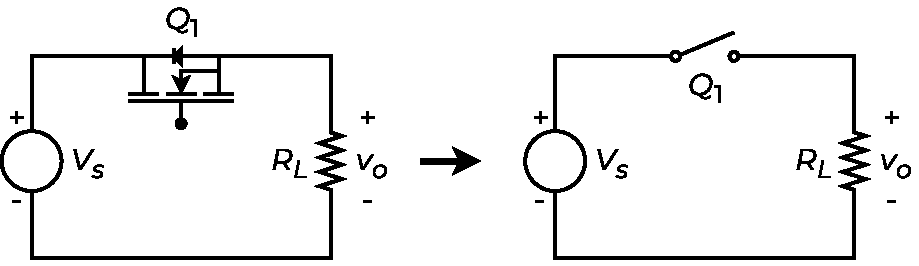
\includegraphics[scale=0.6]{Imagenes/Proto Reductor.pdf}
    \caption{Circuito de un convertidor conmutado básico, y su equivalente con el transistor $Q_1$ como llave ideal.}
    \label{proto_reductor}
\end{figure}

Entonces, si se aplica una señal de control como la de la figura \ref{dutycycle} al interruptor, durante un período $T_s$ de la señal ocurren dos cosas distintas:
"
\begin{itemize}
    \item {\SemiBold Durante el tiempo $\mathbf{t_{on}}$}, el transistor se comporta como una llave cerrada y permite la libre circulación de corriente. Entonces, esta corriente circula por la carga $R_L$, donde, por la Ley de Ohm, cae una tensión igual a la tensión de entrada, es decir, que la tensión de salida {\Medium \textit{v\textsubscript{o}} es igual a la tensión de entrada \textit{V\textsubscript{s}}}.
    \item {\SemiBold Durante el tiempo $\mathbf{t_{off}}$}, el transistor pasa a comportarse como una llave abierta, por lo que restringe completamente la circulación de corriente. Por lo tanto, la caída de tensión en la carga $R_L$ es nula, es decir, que la tensión de salida {\Medium \textit{v\textsubscript{o}} es nula}.
\end{itemize}

Uniendo estos dos comportamientos, se puede ver que la forma de la tensión de salida es análoga a la forma de onda cuadrada que controla al interruptor (de la figura \ref{dutycycle}), oscilando entre \SI{0}{\volt} y $V_s$.

\begin{equation}\label{valor_medio_reductor}
    \bar{v}_o = \frac{1}{T_s}\int\limits^{T_s}_0 v_0(t) dt = \frac{1}{T_s}\int\limits^{DT_s}_0 V_s dt = V_s\cdot D \leq V_s
\end{equation}

Calculando el valor medio de $v_o$ en la ecuación \ref{valor_medio_reductor}, este resulta ser directamente proporcional al ciclo de trabajo de la señal de control, variando entre \SI[]{0}[]{\volt} y la tensión de entrada $V_s$, para ciclos de trabajo entre \num{0} y \num{1} respectivamente. Es decir, la {\Medium tensión media de salida es menor o igual a la de entrada} (esto se puede ver sin necesidad de cálculo, ya que si la salida es igual a la entrada por una proporción del tiempo total, su valor medio necesariamente debe ser menor, o como mucho igual, al valor de la entrada) y se controla directamente con la variación de $D$.\\

En principio, si se considera el transistor como interruptor ideal, la eficiencia de este dispositivo es del 100 \%, ya que durante el tiempo $t_{off}$ no circula ninguna corriente (por lo tanto no hay disipación de ningún tipo), y durante $t_{on}$ no hay caída de tensión en el transistor. En la realidad, los transistores no actúan como llaves ideales, si no que tienen ciertas no idealidades que resultan en pérdidas de energía: no tienen impedancia perfectamente nula como llave cerrada, ni impedancia infinita como llave abierta, además de poseer pérdidas a la hora de conmutar.\\

Sin embargo, en muchos casos y aplicaciones (incluido el de este trabajo) no es suficiente obtener una salida de pulsos y controlar su tensión media, si no que se necesita obtener una tensión puramente continua directamente en la salida, como puede ser el caso para una fuente de alimentación.\\

Para solucionar este problema, se agrega un filtro pasa-bajos LC a la salida luego del interruptor, que se encarga de eliminar los componentes de alta frecuencia relacionados a la conmutación, dejando pasar únicamente los componentes de continua. El convertidor que resulta es la topología de convertidor CC-CC conmutado más sencilla: el {\Medium convertidor reductor} o {\Medium \textit{buck}} de la figura \ref{reductor}, que obtiene su nombre porque, como se ve en la ecuación \ref{valor_medio_reductor}, reduce la tensión de entrada.\\

\begin{figure}[h]
    \centering
    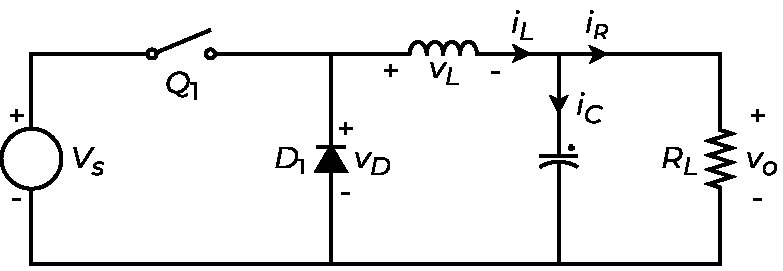
\includegraphics[scale=0.6]{Imagenes/Reductor.pdf}
    \caption{Circuito de un convertidor reductor o buck, con componentes ideales.}
    \label{reductor}
\end{figure}

Además del filtro ya mencionado, se agrega un diodo de rueda libre o \textit{flyback} en derivación entre el transistor y el inductor (diodo $D_1$ de la figura \ref{reductor}). Este dispositivo cumple la función de proveer un camino de circulación para la corriente $i_L$ del inductor cuando el interruptor se encuentra abierto, que resulta necesario ya que la corriente sobre un inductor no puede variar abruptamente. Entonces, cuando el interruptor está abierto, el diodo entra en polarización directa y permite la circulación de corriente; mientras que cuando está el interruptor cerrado, el diodo se polariza con una tensión inversa $V_s$ y actúa como un circuito abierto, eliminando su influencia sobre el convertidor durante $t_{on}$.\\

Durante su funcionamiento en estado estacionario, los convertidores reductores (y todos los convertidores CC-CC) tienen las siguientes propiedades:

\begin{itemize}
    \item La corriente $i_L$ sobre el inductor es periódica de período $T_s$, es decir, $i_L(t+T_s) = i_L(t)$.
    \item La tensión media $\bar{V}_L$ que cae en el inductor es nula, ya que si no lo fuera su corriente crecería sin límite.
    \item La corriente media $\bar{i}_C$ que circula por el capacitor es nula, ya que si no lo fuera su tensión crecería sin límite.
    \item La potencia absorbida por la carga es igual a la potencia entregada por la fuente. Para componentes no ideales, las pérdidas son entregadas por la fuente de entrada.
\end{itemize}

\paragraph{Análisis Detallado}

Ahora se va a realizar un análisis más en profundidad de la topología. Pero antes, es necesario aclarar el conjunto de condiciones que se asumirán, necesarias para simplificar y facilitar la comprensión de esta explicación:

\begin{enumerate}
    \item El circuito opera en estado estacionario, es decir que todos las respuestas transitorias ya se extinguieron.
    \item La corriente del inductor es continua, es decir que circula siempre en la misma dirección.
    \item El capacitor $C$ es lo suficientemente grande como para mantener la tensión de salida constante.
    \item El período de conmutación es $T_s$, con $t_{on} = DT_s$ y $t_{off} = (1-D)T_s$.
    \item Todos los componentes son ideales.
\end{enumerate}

Para poder determinar la tensión de salida $v_o$ del sistema, se va a determinar primero la corriente y tensión del inductor $L$ del filtro de salida, para cada uno de los dos estados del circuito: {\Medium llave abierta} y {\Medium llave cerrada}. Para cumplir la condición de funcionamiento en estado estacionario, la corriente $i_L$ debe tener una variación total nula durante un período $T_s$ (es decir que la corriente debe ser la misma al principio y final de un ciclo), y, como se mencionó más arriba, su tensión media debe ser idénticamente nula.\\

\subparagraph{Llave Cerrada}

Al estar la llave cerrada durante el tiempo $t_{on} = DT_s$, la tensión de entrada $V_s$ cae directamente sobre el diodo $D_1$, polarizándolo con una tensión inversa que no permite que circule corriente por el mismo, y en consecuencia, neutralizando su efecto sobre el circuito. Se puede ver el circuito equivalente para este estado en la figura \ref{reductor_llave_cerrada}.\\

\begin{figure}[h]
    \centering
    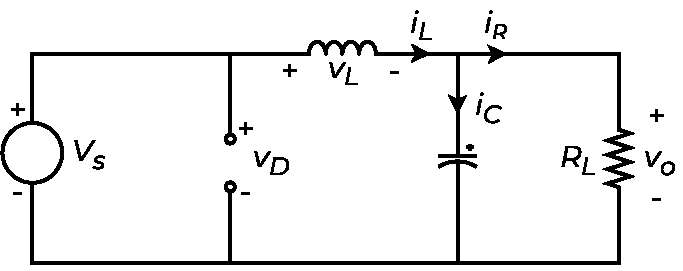
\includegraphics[scale=0.6]{Imagenes/Reductor Llave Cerrada.pdf}
    \caption{Circuito equivalente de un convertidor reductor para llave cerrada.}
    \label{reductor_llave_cerrada}
\end{figure}

Entonces, recordando que la tensión que cae sobre una bobina es proporcional a la corriente que circula sobre ella (con $L$ como constante de proporcionalidad), la tensión sobre el inductor del circuito resulta

\begin{equation}\label{ec_tensionL_cerrada}
    v_L = V_s - v_o = L\frac{di_L}{dt}
\end{equation}

Como la tensión, y por lo tanto la derivada de la corriente, son valores constantes y positivos, la corriente por el inductor es descrita por una recta de pendiente positiva. El cambio neto de corriente $(\Delta i_L)_{cerrado}$ mientras la llave permanece cerrada es entonces

\begin{equation*}
    \frac{di_L}{dt} = \frac{(\Delta i_L)_{cerrado}}{\Delta t} = \frac{(\Delta i_L)_{cerrado}}{DT_s} = \frac{V_s - v_o}{L}\\
\end{equation*}

Reorganizando:

\begin{equation}\label{deltaiL_cerrada}
    \boxed{
        (\Delta i_L)_{cerrado} = \left(\frac{V_s - v_o}{L}\right)DT_s
    }
\end{equation}

\subparagraph{Llave abierta}

Ahora, al abrirse la llave durante el tiempo $t_{off} = (1-D)T_s$, el diodo entra en modo de polarización directa, permitiendo la circulación de la corriente acumulada en el inductor. La fuente queda desconectada y no entrega energía, conformándose el circuito equivalente de la figura \ref{reductor_llave_abierta}.\\

\begin{figure}[h]
    \centering
    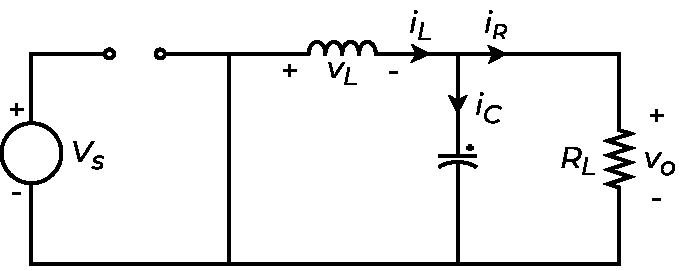
\includegraphics[scale=0.6]{Imagenes/Reductor Llave Abierta.pdf}
    \caption{Circuito equivalente de un convertidor reductor para llave abierta.}
    \label{reductor_llave_abierta}
\end{figure}

En este intervalo de tiempo, la tensión sobre el inductor es

\begin{equation}\label{ec_tensionL_abierta}
    v_L = -v_o = L\frac{di_L}{dt}
\end{equation}

Entonces, aplicando un razonamiento análogo al del período de llave cerrada, con la diferencia que en este caso, al ser la tensión $v_L$ negativa, la recta de la corriente $i_L$ es decreciente, se obtiene que el cambio neto de corriente $(\Delta i_L)_{abierto}$ mientras la llave está abierta es

\begin{equation*}
    \frac{di_L}{dt} = \frac{(\Delta i_L)_{abierto}}{(1-D)T_s} = \frac{-v_o}{L}\\
\end{equation*}

Reordenando:

\begin{equation}\label{deltaiL_abierta}
    \boxed{
        (\Delta i_L)_{abierto} = -\left(\frac{v_o}{L}\right)(1-D)T_s
    }
\end{equation}

Como se mencionó antes, para este análisis se asumió el funcionamiento en estado estacionario, por lo que la suma de los cambios netos de corriente de las ecuaciones \ref{deltaiL_cerrada} y \ref{deltaiL_abierta} para ambos estados del circuito debe ser igual a cero.

\begin{equation}
    (\Delta i_L)_{cerrado} + (\Delta i_L)_{abierto} = 0
\end{equation}

Reemplazando ambas variables por sus expresiones, se obtiene

\begin{equation*}
    \left(\frac{V_s - v_o}{L}\right)DT_s - \left(\frac{v_o}{L}\right)(1-D)T_s  = 0
\end{equation*}

Despejando de la ecuación anterior, se consigue una expresión para la tensión de salida $v_o$ de este convertidor.

\begin{equation}\label{vo_reductor}
    \boxed{
        v_o = V_sD
    }
\end{equation}

Este resultado es idéntico al de la ecuación \ref{valor_medio_reductor} obtenido para el convertidor básico de la figura \ref{proto_reductor}. En conclusión, {\Medium en un convertidor reductor, la tensión de salida siempre es menor o igual a la entrada}.\\

Evidentemente, por el resultado obtenido en la ecuación \ref{vo_reductor}, la salida se controla únicamente con el ciclo de trabajo $D$ del transistor. Por ejemplo, si aumenta la tensión de alimentación $V_s$ pero se desea mantener $v_o$ a un nivel constante, se compensa este aumento con una disminución del ciclo de trabajo (o viceversa). Si se agrega un sensor que mida la tensión de salida, se puede implementar un lazo de control automático que mantiente $v_o$ fijada a una referencia mediante la variación de $D$.\\

\subsubsection{Convertidores CC-CC Aislados}

Habiendo entendido el funcionamiento del convertidor reductor en la anterior sección (que cae en la categoría de convertidores CC-CC no aislados), ahora vamos a pasar a los convertidores CC-CC aislados, categoría en la cual se encuentra el convertidor tipo puente completo de esta plataforma.\\

Los convertidores aislados son generalmente utilizados en fuentes de alimentación de corriente continua, y a diferencia de los no aislados, tienen un transformador de alta frecuencia de por medio, para generar una {\Medium aislación galvánica entre la entrada y la salida}. Además, como los transformadores solo conducen corriente alterna, a su salida debe incluirse algún tipo de circuito rectificador para transformarla a corriente continua para alimentar a la carga.\\

Es claro que el adicionado de un transformador agrega una mayor complejidad al circuito. Entonces, ¿por qué se busca esta aislación galvánica? Sin la aislación interpuesta, nuestra salida va a compartir la conexión a tierra con la fuente de alimentación, (que suelen tener tierras muy ruidosas) introduciendo ruido no deseado a la salida. En muchas aplicaciones hay una gran sensibilidad al ruido en la carga, por lo que es deseable mantenerlo lo más bajo posible, incluso si agrega complejidad al diseño. Adicionalmente, la presencia de aislación galvánica presenta una ventaja en cuestiones de seguridad, tanto para proteger a quienes operan con el circuito como para protección de los componentes del mismo circuito.\\

Otra ventaja es la mayor flexibilidad que un transformador en la etapa de continua aporta al diseño, ya que variando la relación de vueltas entre bobinados (por ejemplo con el uso de múltiples bobinados) se puede variar la tensión de salida entre distintos niveles.\\

Ahora se procederá a derivar las distintas topologías de convertidores aislados, partiendo del convertidor reductor (no aislado) que se explico más arriba. Estos convertidores que obtendremos los vamos a llamar {\Medium convertidores aislados derivados del reductor} o \textit{isolated buck-derived converters}\textsuperscript{\cite{SoftSwitchPWM}}, comenzando por el convertidor \textit{forward}.\\

\paragraph{El Convertidor Forward}

Si tomamos el circuito del reductor de la figura \ref{reductor}, y le agregamos un transformador de alta frecuencia entre la llave $Q_1$ y el diodo $D_1$, se obtiene la aislación galvánica buscada, como se observa en el circuito de la figura \ref{desarrollo_forward}.\\

\begin{figure}[h]
    \centering
    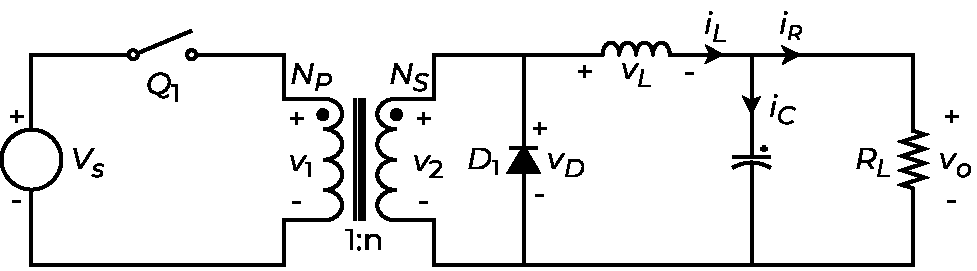
\includegraphics[scale=0.6]{Imagenes/Desarrollo Forward 1.pdf}
    \caption{Convertidor reductor con un transformador interpuesto entre la llave $Q_1$ y el diodo $D_1$.}
    \label{desarrollo_forward}
\end{figure}

Cuando la llave está cerrada, la tensión $V_s$ de entrada se aplica sobre el bobinado primario del transformador, traduciéndose a una tensión de la misma polaridad (por la ubicación de los puntos homólogos) pero afectada por la relación de vueltas $n$. Esto genera que el núcleo ferromagnético del transformador se magnetice, y aumente su flujo de magentización $\phi_m$.\\

Cuando la llave se abre, la corriente del inductor de filtro circula por el diodo $D_1$, cortocircuitando el bobinado secundario del transformador. Esto fuerza que la tensión y la corriente del transformador se anulen, y por lo tanto, el flujo magnetizante se mantiene constante.\\

Entonces, durante un período de conmutación $T_s$, el flujo $\phi_m$ del núcleo del transformador tiene un incremento neto. Pasados suficientes períodos, este flujo aumenta lo suficiente como para saturar el transformador, cosa que no es deseable, ya que puede resultar en corrientes elevadas y eventualmente, la destrucción del transistor de potencia que actúa como llave.\\

Para solucionar este problema, se debe agregar algún circuito auxiliar de restablecimiento del núcleo que, durante el período en el que la llave está abierta, aplique una tensión negativa en el bobinado primario y permita una circulación inversa de corriente para restablecer el flujo magnetizante a su valor original.\\

Pero, al aplicar esta tensión negativa en el primario, se refleja en una tensión negativa del secundario que polariza en directa a $D_1$, cortocircuitando este bobinado. Para arreglar este inconveniente, se puede agregar un diodo rectificador $D_R$ en serie con el bobinado secundario, que no permita la circulación inversa de corriente.\\

Teniendo esto en cuenta, se ve en la figura \ref{forward} el circuito de un {\Medium convertidor \textit{forward}} derivado de un reductor, dónde se agregaron el circuito de restablecimiento de núcleo, compuesto por un bobinado auxiliar y un diodo $D_r$ en serie; en paralelo con el bobinado primario y la llave $Q_1$ (en posiciones invertidas); y el diodo rectificador $D_R$ en el secundario (respecto a la figura \ref{desarrollo_forward}).\\

\begin{figure}[h]
    \centering
    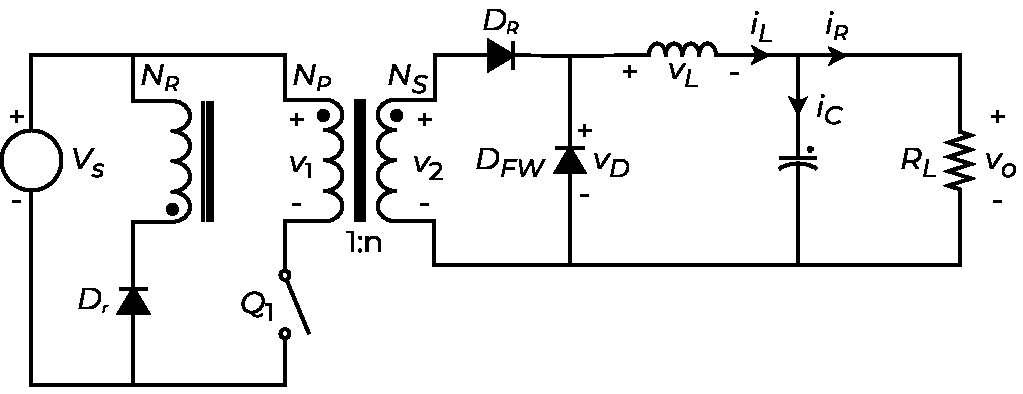
\includegraphics[scale=0.6]{Imagenes/Forward.pdf}
    \caption{Circuito de un convertidor aislado tipo forward, desarrollado a partir del circuito de un reductor.}
    \label{forward}
\end{figure}

Dado que este circuito es similar a un convertidor reductor, solo que con un transformador de relación de vueltas $n$ interpuesto (y los circuitos auxiliares que no afectan la salida), se puede ver que su relación entrada-salida será similar a la del convertidor en el que se basa (ecuación \ref{vo_reductor}) pero afectada por la relación de vueltas del transformador.\textsuperscript{\cite{PotenciaHart}}

\begin{equation}\label{vo_forward}
    \boxed{
        v_o = \left(\frac{N_S}{N_P}\right)V_sD = nV_sD
    }
\end{equation}

Con estos resultados se puede ver la flexibilidad aportada por el transformador: a pesar de ser muy similar a un circuito que solo permite reducir la tensión, con la relación de vueltas se puede obtener cualquier nivel de tensión que se desee a la salida. Sin embargo, al tener que restablecer la magnetización del núcleo, se suele limitar el ciclo de trabajo a 50 \% para poder lograr la demagnetización completa.\\

Además, con el circuito de restablecimiento de flujo, el estrés de tensión sobre la única llave del circuito se duplica respecto al convertidor reductor: al estar la llave abierta, debe soportar una tensión de dos veces la tensión de entrada $V_s$ (para bobinados $N_P$ y $N_R$ iguales). Esto puede ser problemático para aplicaciones de alta tensión, ya que los transistores de alta tensión que se requieren son mas caros y suelen tener desempeño degradado a altas frecuencias de conmutación.\\

\subparagraph{Forward de Doble Llave}

Para solucionar este inconveniente, se puede diseñar un converitdor forward de dos llaves o \textit{double-ended}, que disminuye el estrés de tensión de cada llave a $V_s$ sin cambiar la tensión de salida, que se mantiene igual a la ecuación \ref{vo_forward} del convertidor forward común.\\

Entonces, si agregamos una segunda llave $Q_2$ en serie a la llave original, ambas conmutando al mismo tiempo, la tensión de llave abierta se reparte entre ambas llaves, logrando lo que se buscaba. Para asegurar que en cada llave caiga la tensión $V_s$ correspondiente, se agregan los diodos $D_1$ y $D_2$, conectados entre el terminal negativo del transformador y $V_s$, y entre el terminal negativo de $V_s$ y el terminal positivo del transformador respectivamente.\\

Estos diodos, durante el tiempo en que ninguna llave conduce, permiten el flujo inverso de corriente por el bobinado, cumpliendo el rol adicional de circuito de restablecimiento de $\phi_m$. Esto hace redundante al bobinado $N_R$ y su diodo $D_r$, por lo que se pueden remover, resultando en el circuito de la figura \ref{forward_doubleended}.\\

\begin{figure}[h]
    \centering
    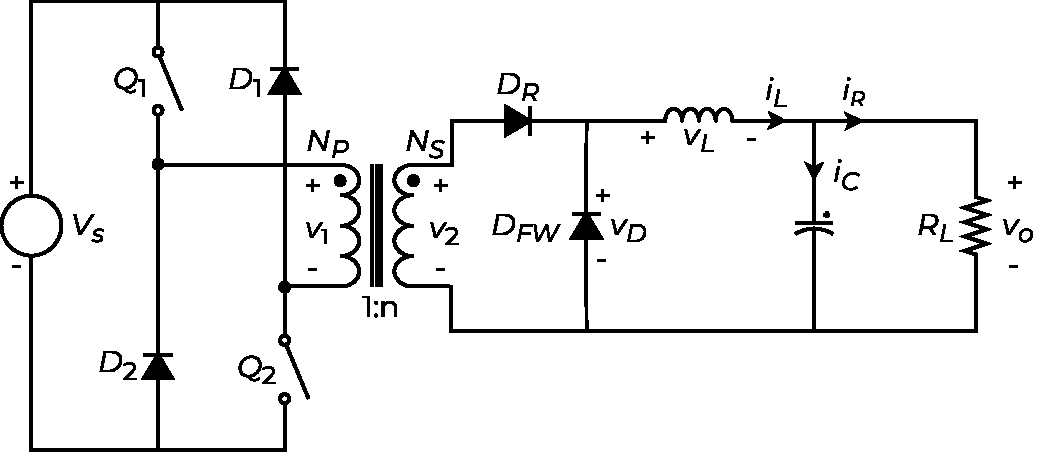
\includegraphics[scale=0.6]{Imagenes/Forward Double-Ended.pdf}
    \caption{Circuito de un convertidor aislado tipo forward de doble llave o double-ended.}
    \label{forward_doubleended}
\end{figure}

Una consecuencia que existe para ambos tipos de convertidores forward (normal y double-ended), es que al estar el ciclo de trabajo limitado a la mitad del período, los requerimientos de filtrado aumentan considerablemente. Esto requiere de la utilización de una bobina de mucha mayor inductancia, aumentando su costo y tamaño, además de introducir una gran cantidad de armónicos de la frecuencia de conmutación.\textsuperscript{\cite{SoftSwitchPWM}}\\

Entonces, se debe encontrar un circuito que sea capaz de obtener una tensión rectificada de secundario que supere el 50 \% de ciclo de trabajo, disminuyendo los requerimientos del filtro y la presencia de armónicos no deseados. Vamos a obtener este circuito partiendo del circuito del convertidor forward de una llave de la figura \ref{forward}.\\

\paragraph{El Convertidor Push-Pull}

Una posible solución podría ser la conexión de dos convertidores forward en paralelo en el primario, que luego compartan el diodo $D_1$ y el filtro de salida LC del lado secundario. Los interruptores $Q_1$ y $Q_2$ deben operar de manera complementaria, con $Q_1$ conduciendo cuando $Q_2$ se abre y viceversa (ambos con el mismo ciclo de trabajo); obteniendo una tensión rectificada del doble de ciclo de trabajo de cada llave.\\

\begin{figure}[h]
    \centering
    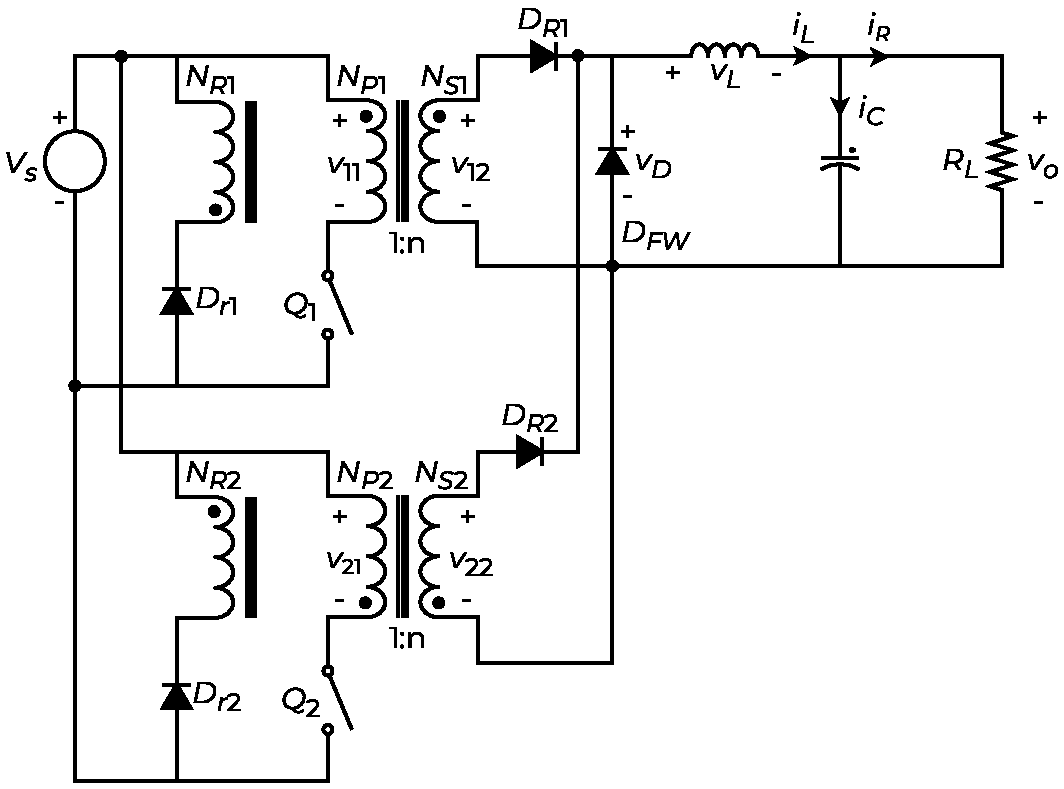
\includegraphics[scale=0.6]{Imagenes/Desarrollo Push-Pull 1.pdf}
    \caption{Dos convertidores forward conectados en paralelo en el primario, compartiendo diodo y filtro de salida.}
    \label{desarrollo_pushpull}
\end{figure}

El circuito resultante de la figura \ref{desarrollo_pushpull}, sin embargo, se puede simplificar. Si hacemos que ambos bobinados primarios compartan su núcleo magnético; entonces, se puede agregar un diodo en antiparalelo a cada llave, de manera que cada uno de estos diodos, junto con los bobinados que tienen en serie, pueden funcionar como circuitos de restablecimiento del núcleo cuando la otra llave esta conduciendo (es decir, cuando $Q_2$ conduce, el diodo antiparalelo de $Q_1$ y su bobinado restablecen la magentización del núcleo, y viceversa).\\

Entonces, los circuitos de restablecimiento heredados del convertidor forward son redundantes, y por lo tanto se pueden remover para simplificar el circuito, resultando en el {\Medium convertidor \textit{push-pull}} que se observa en la figura \ref{pushpull}. Además, el diodo de rueda libre $D_{FW}$ se puede remover, ya que con el rectificador de punto medio conformado por $D_{R1}$ y $D_{R2}$ se forma un camino para la circulación de la corriente del inductor.\\

\begin{figure}[h]
    \centering
    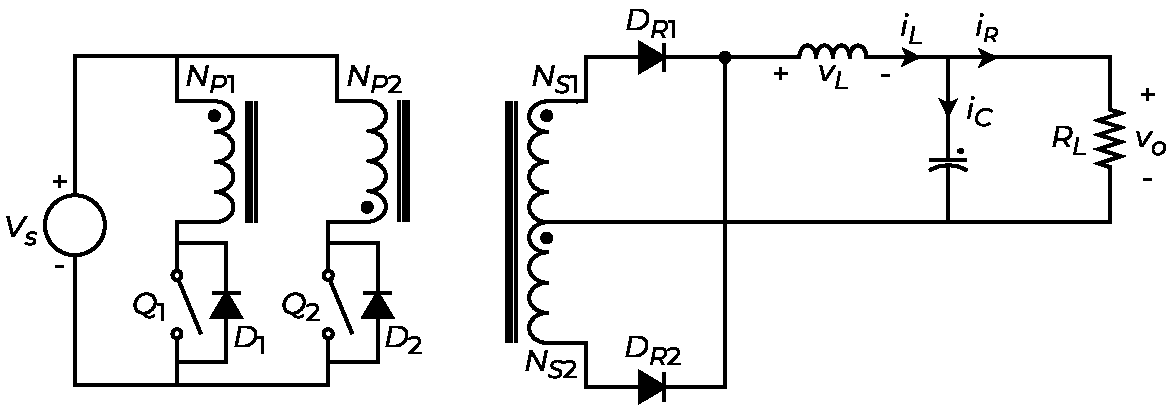
\includegraphics[scale=0.6]{Imagenes/Push-Pull.pdf}
    \caption{Circuito de un convertidor aislado tipo push-pull.}
    \label{pushpull}
\end{figure}

Para obtener su tensión de salida no es necesario realizar toda la deducción matemática. Al ser esta topología esencialmente dos convertidores forward que conducen de manera alternada (cada columna del primario es equivalente a un covertidor forward), el ciclo de trabajo de la onda rectificada es el doble del de cada una de las columnas. Entonces, es razonable decir que su tensión $v_o$ es dos veces la del convertidor forward (ecuación \ref{vo_forward})\textsuperscript{\cite{PotenciaHart}}, siempre que ambos bobinados primarios y secundarios sean iguales.

\begin{equation}\label{vo_pushpull}
    \boxed{
        v_o = 2\left(\frac{N_{S1}}{N_{P1}}\right)V_sD = 2\left(\frac{N_{S2}}{N_{P2}}\right)V_sD
    }
\end{equation}

Esta topología soluciona los problemas de rectificación que tienen los convertidores forward, pero cada llave debe soportar $2V_s$ de tensión cuando está abierta (porque son dos forward intercalados), introduciendo de vuelta la problemática que se solucionó con el forward double-ended. Sería desable entonces, encontrar una topología aislada que sea capaz de solucionar ambos inconvenientes.\\

\subsubsection{El Convertidor de Puente Completo}

Este tipo particular de convertidor aislado, que es el elegido para esta plataforma, es el más complejo dentro de su categoría: utiliza cuatro llaves distintas, y por lo tanto tiene un sobresaliente rendimiento para aplicaciones de alta potencia y tensión. Se va a obtener su circuito a partir de las topologías previamente explicadas, detallando sus ventajas y desventajas. Luego se va a desarrollar un modelo matemático para representarlo y se explicará la forma de controlarlo mediante el método \textit{phase-shift}.\\

Si tomamos el circuito del convertidor forward de dos llaves de la figura \ref{forward_doubleended}, se puede concebir una conxión alternativa para el mismo, donde intercambiamos los lugares de la llave y el diodo en cada una de las dos columnas, e invertimos la posición del punto homólogo del secundario. Entonces, cuando ambas llaves están cerradas (recordando que en esta topología ambas llaves conmutan en conjunto) el núcleo se magnetiza negativamente, y una vez que se abren, lo corriente (positiva) que circula por los diodos restablece los niveles de magnetización.\\

\begin{figure}[h]
    \centering
    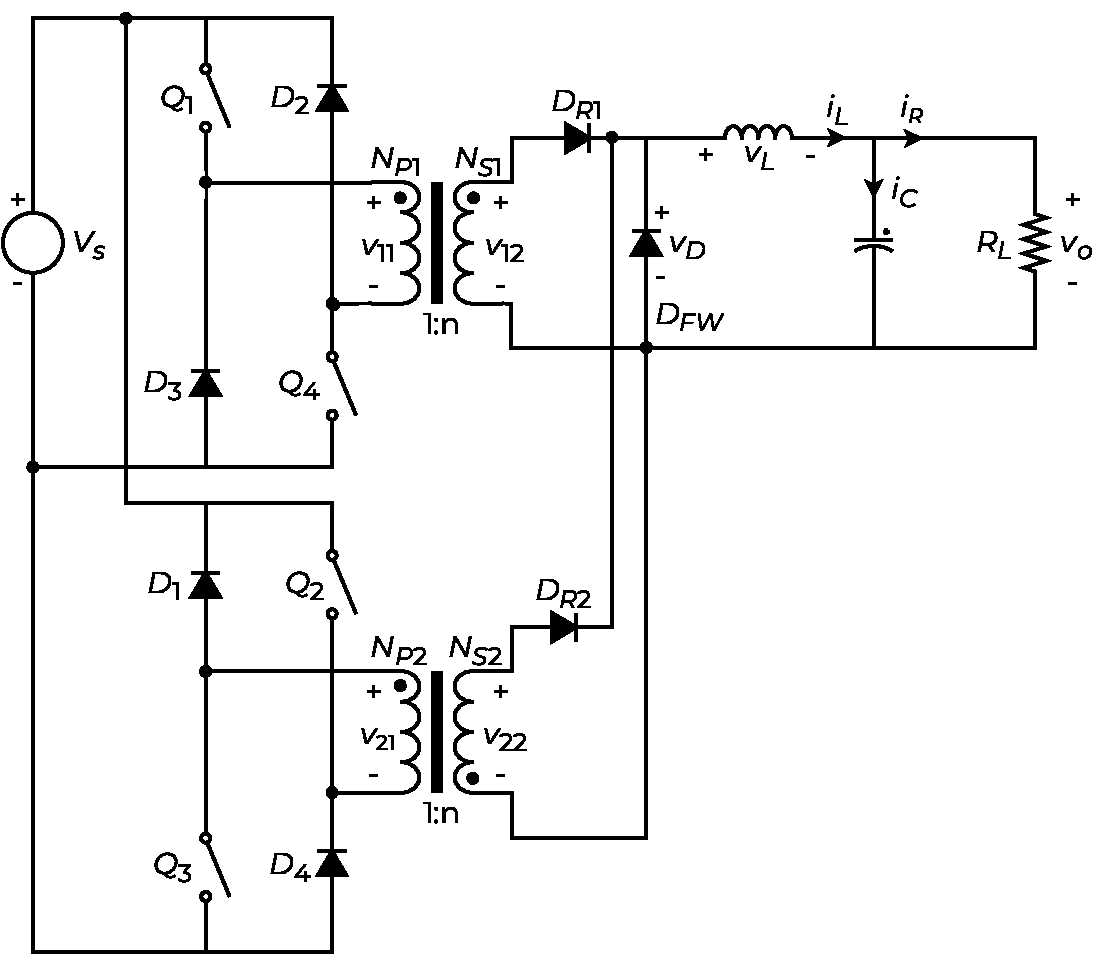
\includegraphics[scale=0.6]{Imagenes/Desarrollo Full-Bridge.pdf}
    \caption{Dos variantes de convertidores forward de dos llaves conectados en paralelo.}
    \label{desarrollo_fullbridge}
\end{figure}

Si conectamos ambas variantes del forward de dos llaves en paralelo, obtenemos el circuito de la figura \ref{desarrollo_fullbridge}, donde las llaves $Q_1$ y $Q_4$ conmutan en sincronía, y desfasadas un tiempo $T_s/2$ de $Q_2$ y $Q_3$ (que también conmutan en sincronía).\\

Siguiendo los pasos de la derivación del push-pull, si hacemos que ambos bobinados primarios compartan un solo núcleo magnético y conectamos diodos antiparalelos a cada una de las llaves, el flujo magnetizante del núcleo puede ser restablecido por los diodos de $Q_1$ y $Q_4$ y el bobinado primario $N_{P1}$, o bien por los diodos de $Q_2$ y $Q_3$ y el bobinado primario $N_{P2}$.\\

Entonces, los diodos $D_1$ a $D_4$ provenientes de los convertidores forward resultan redundantes por la utilización de los diodos antiparalelos, y pueden ser removidos del circuito. Lo que queda entonces, es notar que ahora ambos bobinados primarios tienen formas de onda de tensión y corriente idénticas, por lo que pueden unirse sus terminales positivos y sus terminales negativos, quedando, efectivamente conectados en paralelo. Si ambos bobinados están conectados en paralelo, uno de ellos es redundante y se puede remover sin consecuencias para el funcionamiento del circuito.\\

Si aplicamos todos estos cambios al circuito de la figura \ref{desarrollo_fullbridge}, obtenemos el circuito de un {\Medium convertidor aislado de puente completo} o {\Medium \textit{full-bridge}} en la figura \ref{fullbridge_partido}. Al igual que en el desarrollo del push-pull, el diodo $D_{FW}$ también se puede eliminar ya que los diodos del rectificador de punto medio ya proveen un camino para la corriente del transistor.\\

\begin{figure}[H]
    \centering
    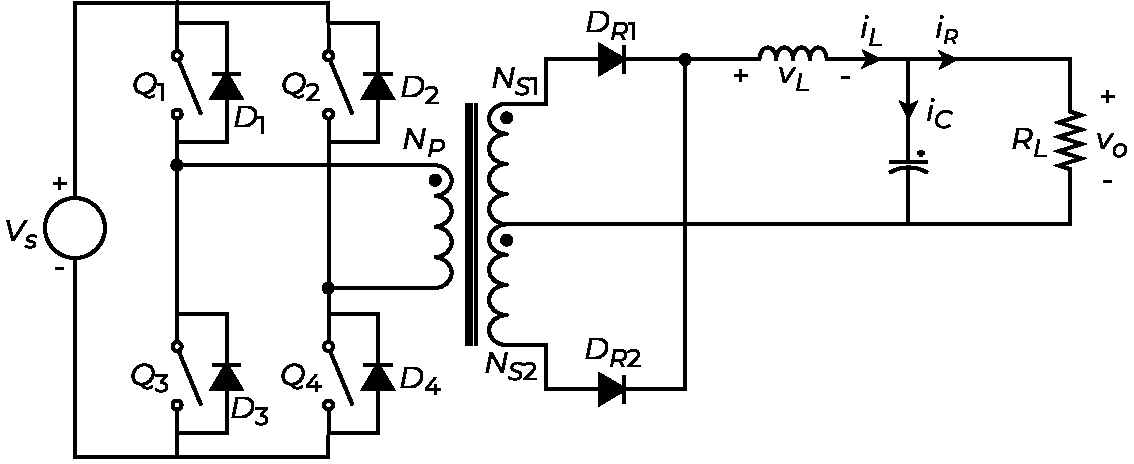
\includegraphics[scale=0.6]{Imagenes/Full Bridge Onda Completa.pdf}
    \caption{Circuito de un convertidor aislado tipo puente completo o full-bridge, con un rectificador de onda completa en el secundario.}
    \label{fullbridge_partido}
\end{figure}

Sin embargo, esta no es la topología exacta que se utiliza en este trabajo. Para simplificar la construcción del transformador de alta frecuencia y disminuir los requerimientos de desempeño impuestos a los diodos rectificadores del secundario, se utiliza un {\Medium rectificador de tipo puente completo} en el secundario como en la figura \ref{fullbridge}. Esta topología utiliza cuatro diodos en vez de dos, pero cada diodo debe soportar la mitad de la tensión inversa. Además, el transformador resulta más sencillo ya que solo tiene un bobinado secundario y no requiere tener punto medio.\\

\begin{figure}[h]
    \centering
    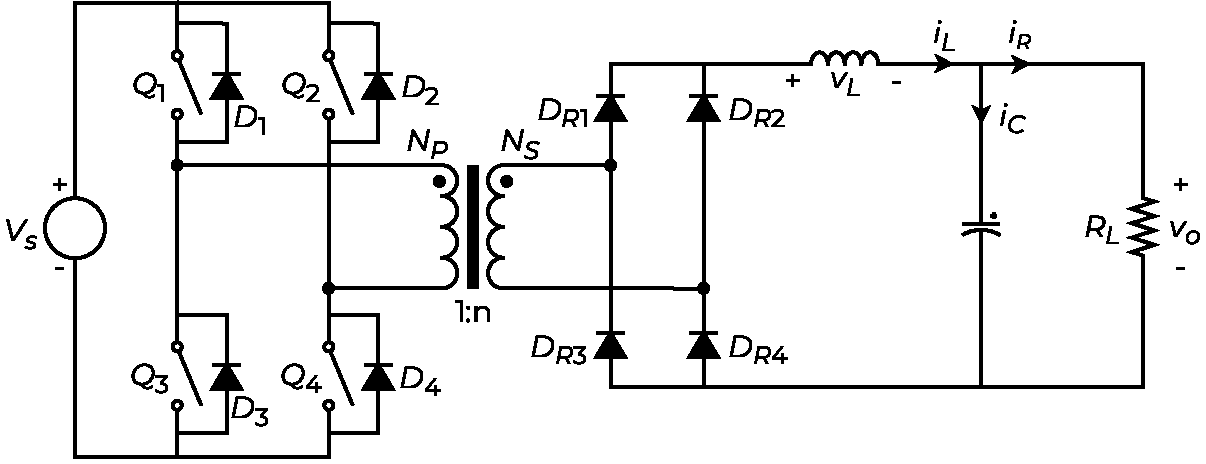
\includegraphics[scale=0.6]{Imagenes/Full Bridge.pdf}
    \caption{Circuito de un convertidor aislado tipo puente completo o full-bridge, con un rectificador de puente completo en el secundario.}
    \label{fullbridge}
\end{figure}

{\Large\Bold\scshape Sección por terminar.}\\


\newpage

\subsection{Sistema de Control}

En forma general, el sistema de control es el bloque de la plataforma que se encarga de tomar los datos de las señales medidas por los distintos sensores, convertirlos a una forma utilizable por el sistema, y luego, mediante un análisis de los mismos, generar señales de comando que se envían al convertidor para modificar su comportamiento, buscando llegar a un punto de funcionamiento adecuado para las condiciones existentes.\\

Todas estas tareas son llevadas a cabo por un dispositivo llamado {\Medium controlador digital de señales} o DSC (del inglés \textit{Digital Signal Controller}). Este dispositivo, como indica su nombre, es un microcontrolador convencional, pero que contiene ciertas modificaciones en su arquitectura de hardware y su repertorio de instrucciones (por ejemplo, hardware dedicado para la operación MAC o \textit{Multiply-and-Accumulate}) que lo adecuan para su uso en el procesamiento de señales digitales.\\

Además, los DSC suelen contar con una gran variedad de periféricos que les brindan flexibilidad para implementar las funcionalidades necesarias para los sistemas en los que se encuentran. Estos periféricos pueden ser módulos de comunicación de datos, contadores y timers, generadores de formas de onda, entre otras cosas. Esta combinación de procesador más periféricos de entrada/salida (y memoria), al implementarse en un sistema más grande y cumpliendo una función dedicada, como es el caso en esta plataforma, resulta en lo que se conoce como {\Medium sistema embebido}.\\

\subsubsection{Controlador Digital de Señales}

Para conformar el sistema embebido de control de la plataforma, se utiliza un controlador digital de señales perteneciente a la linea {\Medium C2000} de microcontroladores de tiempo real de Texas Instruments. En particular, se eligió el modelo {\Medium TMS320F28335} de arquitectura de bus tipo Harvard, \SI[]{150}{\mega\hertz} de frecuencia de reloj, CPU de 32 bits, memoria flash de 256K palabras de 16 bits, conversor analógico-digital de 12 bits y 16 canales, módulos de comunicación serie SPI, I\textsuperscript{2}C, y UART, entre múltiples otras funcionalidades.\textsuperscript{\cite{DSP-Datasheet}}\\

\begin{figure}[h]
    \centering
    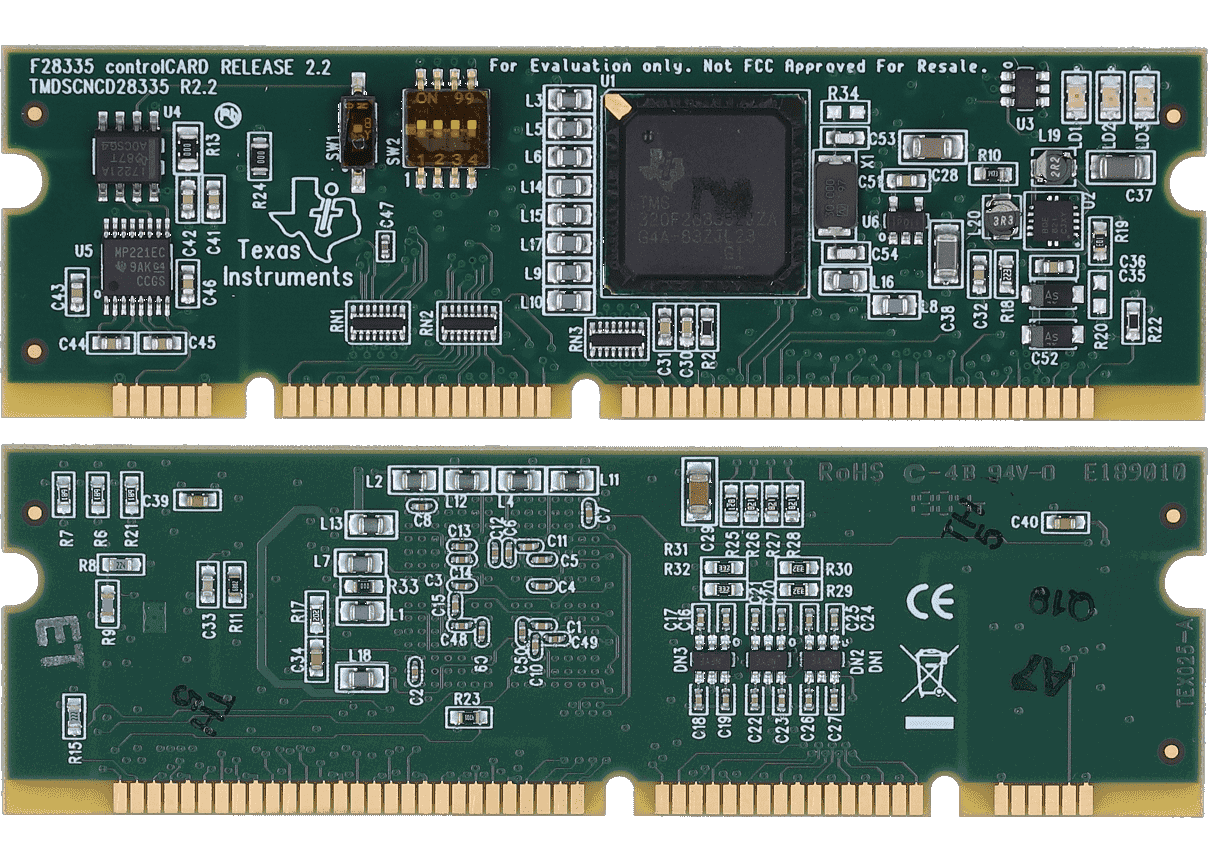
\includegraphics[scale=0.2]{Imagenes/ControlCARD.png}
    \caption{Controlador digital de señales modelo TMS320F28335 de la linea C2000, en su paquete de evaluación tipo ControlCARD, para inserción en slot DIMM-100.}
    \label{ControlCARD}
\end{figure}

Según la hoja de datos que provee el fabricante, este es un DSC optimizado para el procesamiento, sensado y actuación enfocado a mejorar el rendimiento en aplicaciones de control en tiempo real. Cuenta con una unidad de aritmética de punto fijo de 32 bits, además de una FPU (\textit{Floating-Point Unit}) de precisión simple de 32 bits, que le provee una flexibilidad para cumplir tareas tanto de microcontrolador convencional como de procesador de señales digitales. Como se mencionó arriba, tiene capacidad de procesamiento de MAC de 32 x 32 bits con resolución de salida de 64 bits.\textsuperscript{\cite{DSP-Datasheet}}\textsuperscript{\cite{DSP-TechManual}}\\

En tanto a los buses, al ser esta una arquitectura tipo Harvard, el dispositivo cuenta con tres buses separados: un bus de lectura de programa, un bus de lectura de datos y otro bus para la escritura de datos, ambos de 32 bits de ancho. Al estar todos separados, esto permite que se realice la lectura del programa, lectura de datos y escritura de datos en un único ciclo de reloj. Adicionalmente, cuenta con un bus de periféricos que se conecta mediante un \textit{bridge} o puente al bus de memoria principal.\textsuperscript{\cite{DSP-Datasheet}}\textsuperscript{\cite{DSP-TechManual}}\\

El DSC fue seleccionado principalmente por su disponibilidad en el laboratorio, además de que ya fue utilizado en otros proyectos que pueden ser usados como referencia a la hora de diseñar el módulo. En cualquier caso, basado en sus especificaciones, este controlador resulta apropiado para ser integrado al sistema, por su capacidad de procesamiento en tiempo real, su enorme cantidad y variedad de periféricos que permiten implementar diversas funcionalidades útiles, y su documentación muy completa por parte del fabricante.\\

\paragraph{Periféricos Importantes}

Entre la gran lista de periféricos de este dispositivo, se pueden destacar varios de ellos que nos van a resultar de particular interés para la implementación de la plataforma. Estos módulos se conectan a la memoria mediante el bus de periféricos, cada uno con su propio vector de interrupción. Estos son los módulos que nos van a servir principalmente para realizar la adquisición de datos de sensores y la generación de formas de onda de control.

\subparagraph{Módulo ePWM}

El módulo ePWM (\textit{Enhanced Pulse Width Modulator}) del TMS320F28335 cuenta con seis distintos canales de generación de formas de onda por modulación de ancho de pulso desde el ePWM1 hasta el ePWM6, cada uno con dos salidas PWM distintas, ePWMxA y ePWMxB. Todos estos módulos pueden ser unidos mediante un esquema de sincronización por reloj si se requiere que operen como un único sistema.\\

\begin{figure}[h]
    \centering
    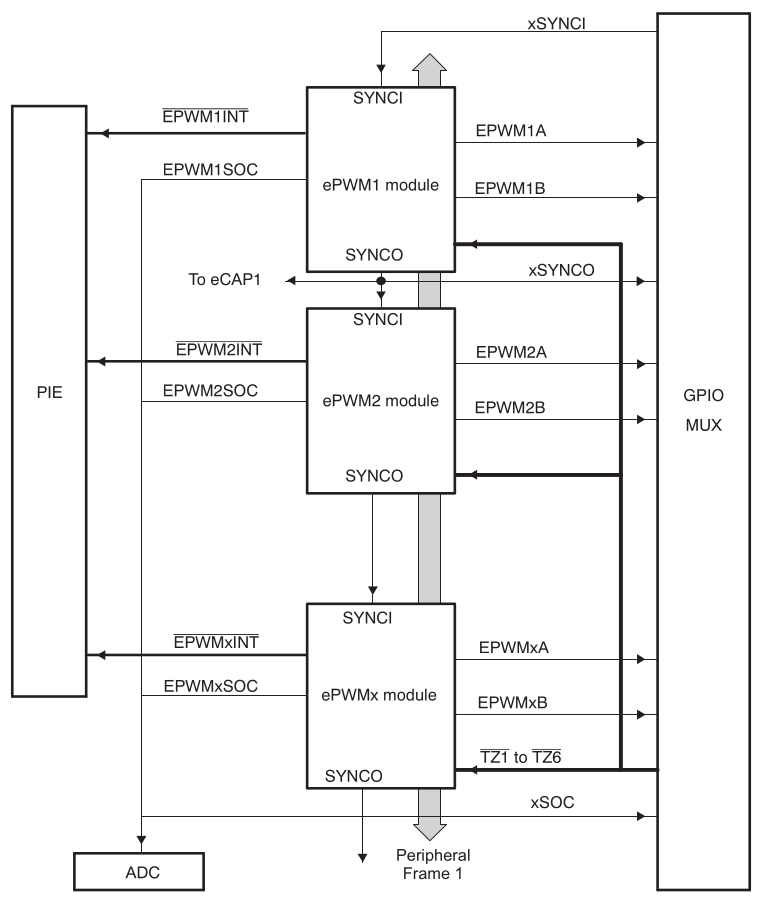
\includegraphics[scale=0.3]{Imagenes/Modulo ePWM.png}
    \caption{Diagrama de conexión interna de los módulos ePWM dentro del dispositivo.\textsuperscript{\cite{DSP-TechManual}}}
    \label{Modulo-ePWM}
\end{figure}

La frecuencia y fase de las ondas de cada uno de los módulos son controladas por un timer de 16 bits de longitud, con un \textit{prescaler} que permite modificar la base de tiempo mediante la división de frecuencia del reloj de entrada. Las salidas A y B de cada módulo se pueden configurar en tres modos: dos salidas independientes de operación flanco simple, dos salidas independientes de operación flanco dual simétricas, y una salida de operación flanco dual asimétrica.\\

Como se ve en la figura \ref{Modulo-ePWM}, cada módulo cuenta con una entrada de sincronización SYNCI y salida de sincronización SYNCO. Esto permite encadenar dos módulos, con la señal de sincronización de un módulo proveniente de otro módulo anterior. Además, cada módulo cuenta con un registro de fase de 16 bits, cuyo contenido define la fase de las ondas generadas respecto a las ondas del módulo del cual esta recibiendo la señal de sincronización (esto va a resultar útil para generar las señales de comando del convertidor full-brigde de la plataforma).\\

Adicionalmente, cada módulo ePWM cuenta con un submódulo de generación de banda muerta o \textit{dead-band} para flancos de subida y bajada. Esto permite generar un período de tiempo muerto (es decir, un tiempo en el que no se cambia de nivel) entre flancos de las salidas A y B del módulo. Esto resulta útil en convertidores puente, como función de seguridad para evitar el disparo simultáneo de las dos llaves de una pata.\textsuperscript{\cite{DSP-TechManual}}\\

\subparagraph{Módulo ADC}

El TMS320F28335 cuenta con un conversor analógico-digital de 12 bits (4096 niveles) de resolución y 16 canales, configurables como dos módulos independientes de 8 canales cada uno (ADCINAx y ADCINBx).\\

\begin{figure}[h]
    \centering
    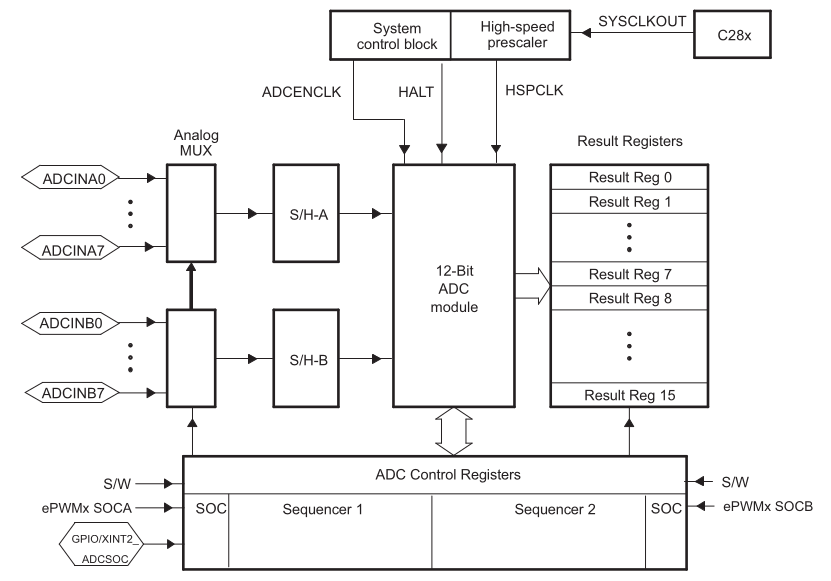
\includegraphics[scale=0.35]{Imagenes/Modulo ADC.png}
    \caption{Diagrama de la conexión interna del módulo de conversor analógico-digital del dispositivo.\textsuperscript{\cite{DSP-TechManual}}}
    \label{Modulo-ADC}
\end{figure}

Como se ve en la figura \ref{Modulo-ADC}, existe un único conversor en el cual las entradas analógicas ingresan a través de un circuito multiplexor analógico. Cada uno de estos multiplexores (uno para cada grupo A y B) tiene a continuación un circuito de \textit{Sample and Hold}, que se encarga de mantener el nivel de tensión de entrada fijo en el valor correspondiente al instante en el que se tomó la muestra para que se pueda realizar la conversión. Luego, el conversor toma valores de tensión entre \SI[]{0.0}{\volt} y \SI[]{3.0}{\volt}, convirtiendolos a una velocidad de \num[]{12.5} MSPS (período de conversión de \SI[]{80}{\nano\second}).\\

Además, existen múltiples posibles fuentes para la secuencia de inicio de conversión (SOC): inicio inmediato por software, inicio mediante señal ePWM, e inicio mediante la interrupción externa XINT2.\textsuperscript{\cite{DSP-Datasheet}}\\

\newpage

\subsection{Carga Electrónica Variable}

Para la realización de los ensayos necesarios para relevar el funcionamiento de la plataforma, se debe contar con algún tipo de carga a la salida del sistema que se encargue de absorber la potencia entregada en la entrada por el emulador de pilas de combustible. Debe ser una carga programable o variable, que permita evaluar el funcionamiento del sistema en las distintas condiciones de carga que se puedan encontrar en un sistema híbrido.\\

El modelo seleccionado para cumplir este rol es la carga programable de corriente continua disponible en el laboratorio, modelo {\Medium IT8514B+} del fabricante ITECH Electronic, que se puede observar en la figura a continuación.\\

\begin{figure}[h]
    \centering
    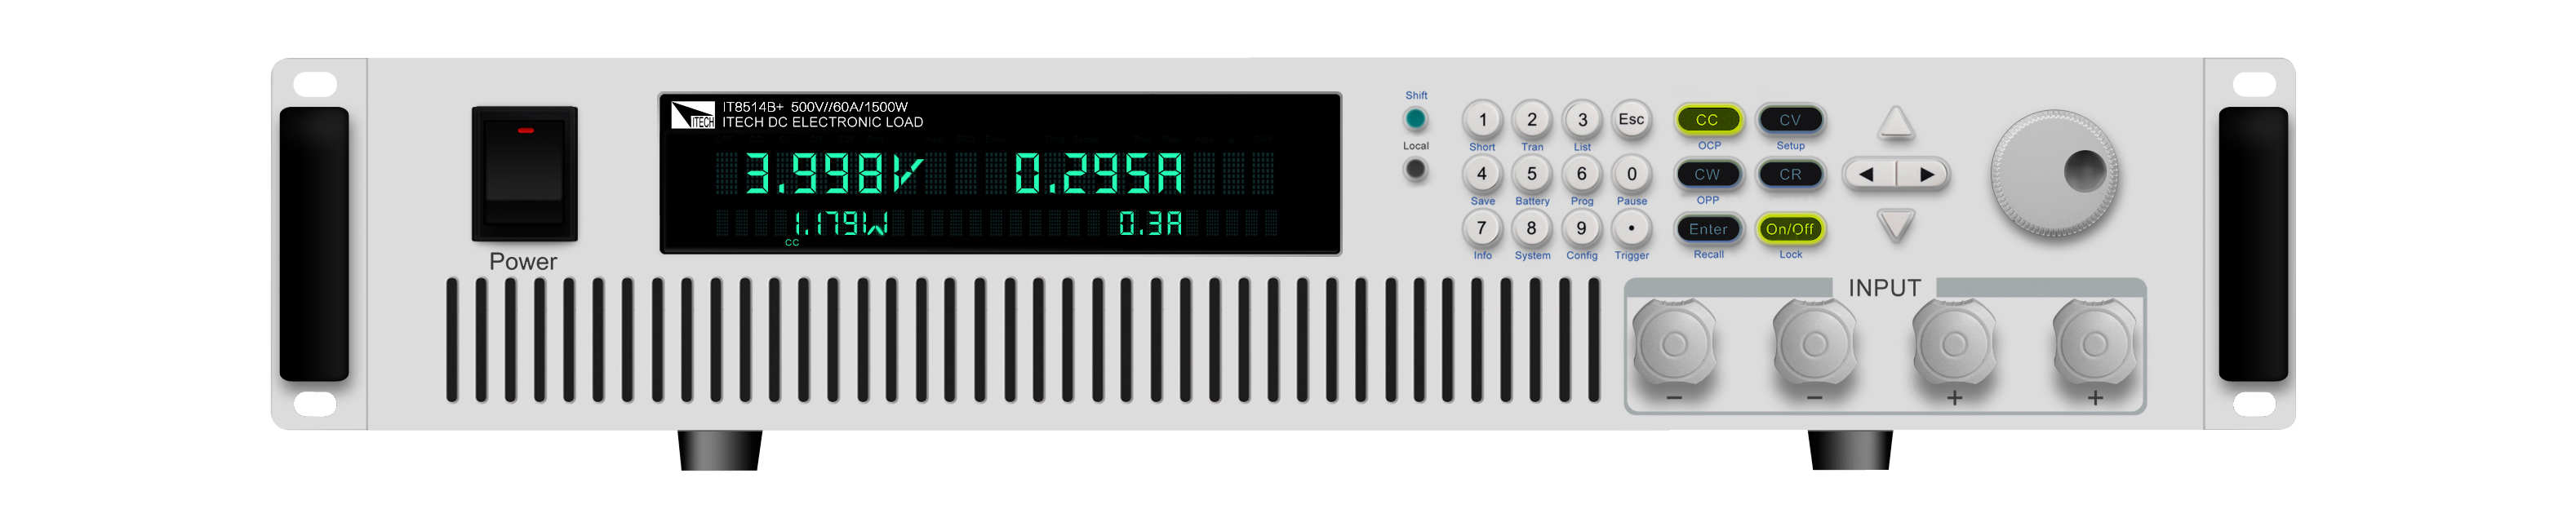
\includegraphics[scale=0.55]{Imagenes/Carga Variable.png}
    \caption{Carga electrónica variable disponible en el laboratorio, modelo ITECH IT8514B+.}
    \label{carga_variable}
\end{figure}

Esta carga programable cuenta con cuatro modos distintos de emulación de carga: corriente constante (CC) hasta \SI[]{60}{\ampere}, tensión constante (CV) hasta \SI[]{500}{\volt}, resistencia constante (CR) y potencia constante (CW) hasta \SI[]{1500}{\watt}. Como se puede ver en la figura \ref{carga_variable}, el dispositivo cuenta con un display en el cuál se indican los valores de tensión, corriente y potencia absorbidos por la carga con alta precisión, evitando la necesidad de utilizar un dispositivo de medida separado para obtener estas figuras.\textsuperscript{\cite{CargaVariable}}\\

Adicionalmente cuenta con modo transitorio, que permite conmutar periódicamente entre dos niveles de carga distintos; y modo de lista, que da la opción de generar una secuencia compleja de niveles de carga, con opciones de sincronización externa e interna.\textsuperscript{\cite{CargaVariable}}\\

Todas estas funcionalidades, junto con su capacidad de tensión, corriente y potencia elevadas, hacen a este un dispositivo ideal para la evaluación del funcionamiento de la plataforma en todas las condiciones de carga necesarias.\\

\newpage

\subsection{Resumen}

\lipsum[1]\\

\lipsum[2]\\

\newpage

    \newpage
    \thispagestyle{plain}
    \printbibliography[heading=bibintoc,title={Referencias}]
    
\end{document}